\documentclass[twoside]{book}

% Packages required by doxygen
\usepackage{fixltx2e}
\usepackage{calc}
\usepackage{doxygen}
\usepackage[export]{adjustbox} % also loads graphicx
\usepackage{graphicx}
\usepackage[utf8]{inputenc}
\usepackage{makeidx}
\usepackage{multicol}
\usepackage{multirow}
\PassOptionsToPackage{warn}{textcomp}
\usepackage{textcomp}
\usepackage[nointegrals]{wasysym}
\usepackage[table]{xcolor}

% Font selection
\usepackage[T1]{fontenc}
\usepackage[scaled=.90]{helvet}
\usepackage{courier}
\usepackage{amssymb}
\usepackage{sectsty}
\renewcommand{\familydefault}{\sfdefault}
\allsectionsfont{%
  \fontseries{bc}\selectfont%
  \color{darkgray}%
}
\renewcommand{\DoxyLabelFont}{%
  \fontseries{bc}\selectfont%
  \color{darkgray}%
}
\newcommand{\+}{\discretionary{\mbox{\scriptsize$\hookleftarrow$}}{}{}}

% Page & text layout
\usepackage{geometry}
\geometry{%
  a4paper,%
  top=2.5cm,%
  bottom=2.5cm,%
  left=2.5cm,%
  right=2.5cm%
}
\tolerance=750
\hfuzz=15pt
\hbadness=750
\setlength{\emergencystretch}{15pt}
\setlength{\parindent}{0cm}
\setlength{\parskip}{0.2cm}
\makeatletter
\renewcommand{\paragraph}{%
  \@startsection{paragraph}{4}{0ex}{-1.0ex}{1.0ex}{%
    \normalfont\normalsize\bfseries\SS@parafont%
  }%
}
\renewcommand{\subparagraph}{%
  \@startsection{subparagraph}{5}{0ex}{-1.0ex}{1.0ex}{%
    \normalfont\normalsize\bfseries\SS@subparafont%
  }%
}
\makeatother

% Headers & footers
\usepackage{fancyhdr}
\pagestyle{fancyplain}
\fancyhead[LE]{\fancyplain{}{\bfseries\thepage}}
\fancyhead[CE]{\fancyplain{}{}}
\fancyhead[RE]{\fancyplain{}{\bfseries\leftmark}}
\fancyhead[LO]{\fancyplain{}{\bfseries\rightmark}}
\fancyhead[CO]{\fancyplain{}{}}
\fancyhead[RO]{\fancyplain{}{\bfseries\thepage}}
\fancyfoot[LE]{\fancyplain{}{}}
\fancyfoot[CE]{\fancyplain{}{}}
\fancyfoot[RE]{\fancyplain{}{\bfseries\scriptsize Generated on Sun Nov 8 2015 23\+:58\+:15 for My Project by Doxygen }}
\fancyfoot[LO]{\fancyplain{}{\bfseries\scriptsize Generated on Sun Nov 8 2015 23\+:58\+:15 for My Project by Doxygen }}
\fancyfoot[CO]{\fancyplain{}{}}
\fancyfoot[RO]{\fancyplain{}{}}
\renewcommand{\footrulewidth}{0.4pt}
\renewcommand{\chaptermark}[1]{%
  \markboth{#1}{}%
}
\renewcommand{\sectionmark}[1]{%
  \markright{\thesection\ #1}%
}

% Indices & bibliography
\usepackage{natbib}
\usepackage[titles]{tocloft}
\setcounter{tocdepth}{3}
\setcounter{secnumdepth}{5}
\makeindex

% Hyperlinks (required, but should be loaded last)
\usepackage{ifpdf}
\ifpdf
  \usepackage[pdftex,pagebackref=true]{hyperref}
\else
  \usepackage[ps2pdf,pagebackref=true]{hyperref}
\fi
\hypersetup{%
  colorlinks=true,%
  linkcolor=blue,%
  citecolor=blue,%
  unicode%
}

% Custom commands
\newcommand{\clearemptydoublepage}{%
  \newpage{\pagestyle{empty}\cleardoublepage}%
}


%===== C O N T E N T S =====

\begin{document}

% Titlepage & ToC
\hypersetup{pageanchor=false,
             bookmarks=true,
             bookmarksnumbered=true,
             pdfencoding=unicode
            }
\pagenumbering{roman}
\begin{titlepage}
\vspace*{7cm}
\begin{center}%
{\Large My Project }\\
\vspace*{1cm}
{\large Generated by Doxygen 1.8.10}\\
\vspace*{0.5cm}
{\small Sun Nov 8 2015 23:58:15}\\
\end{center}
\end{titlepage}
\clearemptydoublepage
\tableofcontents
\clearemptydoublepage
\pagenumbering{arabic}
\hypersetup{pageanchor=true}

%--- Begin generated contents ---
\chapter{Hierarchical Index}
\section{Class Hierarchy}
This inheritance list is sorted roughly, but not completely, alphabetically\+:\begin{DoxyCompactList}
\item \contentsline{section}{Auto\+Repair\+Shop}{\pageref{class_auto_repair_shop}}{}
\item \contentsline{section}{Config\+File}{\pageref{class_config_file}}{}
\begin{DoxyCompactList}
\item \contentsline{section}{Auto\+Repair\+Shop\+File}{\pageref{class_auto_repair_shop_file}}{}
\item \contentsline{section}{Clients\+File}{\pageref{class_clients_file}}{}
\item \contentsline{section}{Employees\+File}{\pageref{class_employees_file}}{}
\item \contentsline{section}{Vehicles\+File}{\pageref{class_vehicles_file}}{}
\end{DoxyCompactList}
\item \contentsline{section}{Date}{\pageref{struct_date}}{}
\item \contentsline{section}{Config\+File\+:\+:Empty\+File\+Exception}{\pageref{class_config_file_1_1_empty_file_exception}}{}
\item \contentsline{section}{Config\+File\+:\+:File\+Exception}{\pageref{class_config_file_1_1_file_exception}}{}
\begin{DoxyCompactList}
\item \contentsline{section}{Config\+File\+:\+:Bad\+File\+Exception}{\pageref{class_config_file_1_1_bad_file_exception}}{}
\item \contentsline{section}{Config\+File\+:\+:Inexistent\+File\+Exception}{\pageref{class_config_file_1_1_inexistent_file_exception}}{}
\end{DoxyCompactList}
\item \contentsline{section}{Auto\+Repair\+Shop\+:\+:Inexistent\+Vehicle}{\pageref{class_auto_repair_shop_1_1_inexistent_vehicle}}{}
\item \contentsline{section}{Person}{\pageref{class_person}}{}
\begin{DoxyCompactList}
\item \contentsline{section}{Client}{\pageref{class_client}}{}
\item \contentsline{section}{Employee}{\pageref{class_employee}}{}
\end{DoxyCompactList}
\item \contentsline{section}{Service}{\pageref{class_service}}{}
\begin{DoxyCompactList}
\item \contentsline{section}{Non\+Standard\+Service}{\pageref{class_non_standard_service}}{}
\item \contentsline{section}{Standard\+Service}{\pageref{class_standard_service}}{}
\begin{DoxyCompactList}
\item \contentsline{section}{Car\+Wash}{\pageref{class_car_wash}}{}
\item \contentsline{section}{Inspection}{\pageref{class_inspection}}{}
\item \contentsline{section}{Oil\+Change}{\pageref{class_oil_change}}{}
\end{DoxyCompactList}
\end{DoxyCompactList}
\item \contentsline{section}{Vehicle}{\pageref{class_vehicle}}{}
\begin{DoxyCompactList}
\item \contentsline{section}{Automobile}{\pageref{class_automobile}}{}
\item \contentsline{section}{Bus}{\pageref{class_bus}}{}
\item \contentsline{section}{Motorcycle}{\pageref{class_motorcycle}}{}
\item \contentsline{section}{Truck}{\pageref{class_truck}}{}
\end{DoxyCompactList}
\end{DoxyCompactList}

\chapter{Class Index}
\section{Class List}
Here are the classes, structs, unions and interfaces with brief descriptions\+:\begin{DoxyCompactList}
\item\contentsline{section}{\hyperlink{class_automobile}{Automobile} }{\pageref{class_automobile}}{}
\item\contentsline{section}{\hyperlink{class_auto_repair_shop}{Auto\+Repair\+Shop} \\*Main class of the project, contains info of all vehicles, employees and clients on it }{\pageref{class_auto_repair_shop}}{}
\item\contentsline{section}{\hyperlink{class_auto_repair_shop_file}{Auto\+Repair\+Shop\+File} \\*Name of the vehiclesfile, clientsfile and employeesfile and the name of the Auto Repair Shop }{\pageref{class_auto_repair_shop_file}}{}
\item\contentsline{section}{\hyperlink{class_config_file_1_1_bad_file_exception}{Config\+File\+::\+Bad\+File\+Exception} }{\pageref{class_config_file_1_1_bad_file_exception}}{}
\item\contentsline{section}{\hyperlink{class_bus}{Bus} }{\pageref{class_bus}}{}
\item\contentsline{section}{\hyperlink{class_car_wash}{Car\+Wash} }{\pageref{class_car_wash}}{}
\item\contentsline{section}{\hyperlink{class_client}{Client} \\*Subclass of \hyperlink{class_person}{Person}, someone with cars on the Auto Repair Shop }{\pageref{class_client}}{}
\item\contentsline{section}{\hyperlink{class_clients_file}{Clients\+File} \\*Info of all the clients of the Auto Repair Shop }{\pageref{class_clients_file}}{}
\item\contentsline{section}{\hyperlink{class_config_file}{Config\+File} \\*Superclass to all types of file Keeps their common behaviour }{\pageref{class_config_file}}{}
\item\contentsline{section}{\hyperlink{struct_date}{Date} }{\pageref{struct_date}}{}
\item\contentsline{section}{\hyperlink{class_employee}{Employee} \\*Subclass of \hyperlink{class_person}{Person}, responsible by cars on the Auto Repair Shop }{\pageref{class_employee}}{}
\item\contentsline{section}{\hyperlink{class_employees_file}{Employees\+File} }{\pageref{class_employees_file}}{}
\item\contentsline{section}{\hyperlink{class_config_file_1_1_empty_file_exception}{Config\+File\+::\+Empty\+File\+Exception} }{\pageref{class_config_file_1_1_empty_file_exception}}{}
\item\contentsline{section}{\hyperlink{class_config_file_1_1_file_exception}{Config\+File\+::\+File\+Exception} }{\pageref{class_config_file_1_1_file_exception}}{}
\item\contentsline{section}{\hyperlink{class_config_file_1_1_inexistent_file_exception}{Config\+File\+::\+Inexistent\+File\+Exception} }{\pageref{class_config_file_1_1_inexistent_file_exception}}{}
\item\contentsline{section}{\hyperlink{class_auto_repair_shop_1_1_inexistent_vehicle}{Auto\+Repair\+Shop\+::\+Inexistent\+Vehicle} }{\pageref{class_auto_repair_shop_1_1_inexistent_vehicle}}{}
\item\contentsline{section}{\hyperlink{class_inspection}{Inspection} }{\pageref{class_inspection}}{}
\item\contentsline{section}{\hyperlink{class_motorcycle}{Motorcycle} }{\pageref{class_motorcycle}}{}
\item\contentsline{section}{\hyperlink{class_non_standard_service}{Non\+Standard\+Service} \\*Non Standard Services Performed on Vehicles }{\pageref{class_non_standard_service}}{}
\item\contentsline{section}{\hyperlink{class_oil_change}{Oil\+Change} \\*Oil Change \hyperlink{class_service}{Service} Performed on Vehicles }{\pageref{class_oil_change}}{}
\item\contentsline{section}{\hyperlink{class_person}{Person} \\*Superclass to \hyperlink{class_employee}{Employee} and \hyperlink{class_client}{Client} }{\pageref{class_person}}{}
\item\contentsline{section}{\hyperlink{class_service}{Service} \\*Superclass to \hyperlink{class_standard_service}{Standard\+Service} and \hyperlink{class_non_standard_service}{Non\+Standard\+Service} }{\pageref{class_service}}{}
\item\contentsline{section}{\hyperlink{class_standard_service}{Standard\+Service} \\*Superclass to \hyperlink{class_oil_change}{Oil\+Change}, \hyperlink{class_inspection}{Inspection} and \hyperlink{class_car_wash}{Car\+Wash} }{\pageref{class_standard_service}}{}
\item\contentsline{section}{\hyperlink{class_truck}{Truck} }{\pageref{class_truck}}{}
\item\contentsline{section}{\hyperlink{class_vehicle}{Vehicle} \\*Superclass to \hyperlink{class_automobile}{Automobile}, \hyperlink{class_motorcycle}{Motorcycle}, \hyperlink{class_truck}{Truck} and \hyperlink{class_bus}{Bus} }{\pageref{class_vehicle}}{}
\item\contentsline{section}{\hyperlink{class_vehicles_file}{Vehicles\+File} \\*Info of all the vehicles on the Auto Repair Shop }{\pageref{class_vehicles_file}}{}
\end{DoxyCompactList}

\chapter{Class Documentation}
\hypertarget{class_automobile}{}\section{Automobile Class Reference}
\label{class_automobile}\index{Automobile@{Automobile}}
Inheritance diagram for Automobile\+:\begin{figure}[H]
\begin{center}
\leavevmode
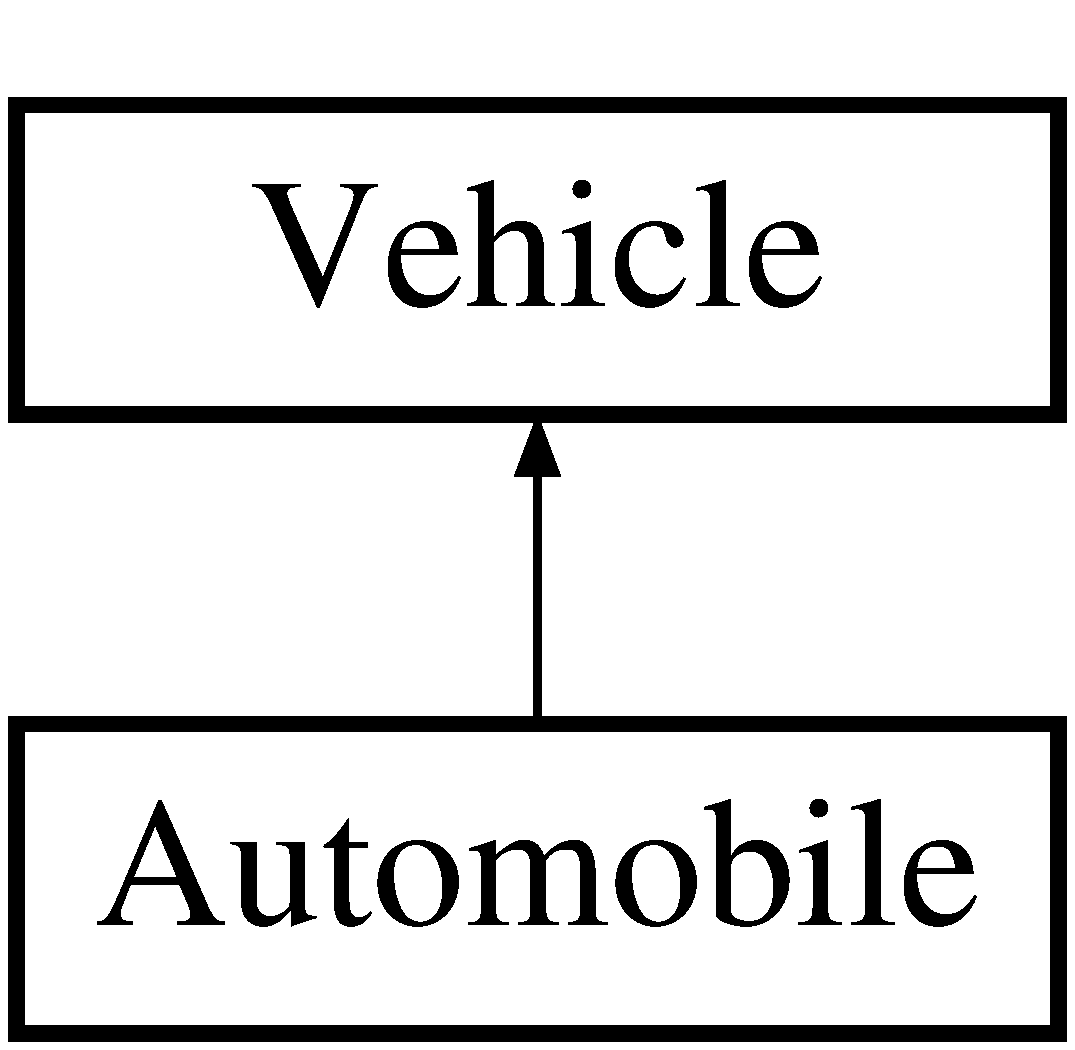
\includegraphics[height=2.000000cm]{class_automobile}
\end{center}
\end{figure}
\subsection*{Public Member Functions}
\begin{DoxyCompactItemize}
\item 
\hypertarget{class_automobile_a50de91a49a5e647f4fddc81448bbd764}{}{\bfseries Automobile} (string manufacturer, string model, string license\+Plate, int num\+Doors)\label{class_automobile_a50de91a49a5e647f4fddc81448bbd764}

\item 
\hypertarget{class_automobile_a2b19291f5f88159eebd8432cb648ec78}{}{\bfseries Automobile} (istream \&in)\label{class_automobile_a2b19291f5f88159eebd8432cb648ec78}

\item 
\hypertarget{class_automobile_a77ef785be9cd16cef586c7caaf44ae6a}{}int {\bfseries class\+Identifier} ()\label{class_automobile_a77ef785be9cd16cef586c7caaf44ae6a}

\item 
\hypertarget{class_automobile_a57f35aee6f148238bd958bd7e348700f}{}void {\bfseries save\+Object\+Info} (ostream \&out)\label{class_automobile_a57f35aee6f148238bd958bd7e348700f}

\item 
\hypertarget{class_automobile_adf6a4503cb73f9d8a0fb588c2c472540}{}void {\bfseries print\+Object\+Info} () const \label{class_automobile_adf6a4503cb73f9d8a0fb588c2c472540}

\end{DoxyCompactItemize}


The documentation for this class was generated from the following files\+:\begin{DoxyCompactItemize}
\item 
Vehicle.\+h\item 
Vehicle.\+cpp\end{DoxyCompactItemize}

\hypertarget{class_auto_repair_shop}{}\section{Auto\+Repair\+Shop Class Reference}
\label{class_auto_repair_shop}\index{Auto\+Repair\+Shop@{Auto\+Repair\+Shop}}


main class of the project, contains info of all vehicles, employees and clients on it  




{\ttfamily \#include $<$Auto\+Repair\+Shop.\+h$>$}

\subsection*{Classes}
\begin{DoxyCompactItemize}
\item 
class \hyperlink{class_auto_repair_shop_1_1_inexistent_vehicle}{Inexistent\+Vehicle}
\end{DoxyCompactItemize}
\subsection*{Public Member Functions}
\begin{DoxyCompactItemize}
\item 
\hypertarget{class_auto_repair_shop_abfd899870a9e0840ce888f8cfad6cb4c}{}\hyperlink{class_auto_repair_shop_abfd899870a9e0840ce888f8cfad6cb4c}{Auto\+Repair\+Shop} (string name)\label{class_auto_repair_shop_abfd899870a9e0840ce888f8cfad6cb4c}

\begin{DoxyCompactList}\small\item\em creates an object of \hyperlink{class_auto_repair_shop}{Auto\+Repair\+Shop} class \end{DoxyCompactList}\item 
bool \hyperlink{class_auto_repair_shop_a51b51e852827d936df828b34abc19eaf}{is\+Client} (\hyperlink{class_client}{Client} client1)
\item 
bool \hyperlink{class_auto_repair_shop_a9d1534c8de54c5a34958e04222c4a93b}{is\+Employee} (\hyperlink{class_employee}{Employee} employee1)
\item 
bool \hyperlink{class_auto_repair_shop_ab7141a5910487566c637497dcef4c26c}{add\+Client} (\hyperlink{class_client}{Client} client)
\begin{DoxyCompactList}\small\item\em adds client to the clients vector if he wasn\textquotesingle{}t there \end{DoxyCompactList}\item 
bool \hyperlink{class_auto_repair_shop_a8e5171bd079137114eba615753a07a82}{add\+Employee} (\hyperlink{class_employee}{Employee} employee)
\begin{DoxyCompactList}\small\item\em adds employee to the employees vector if he wasn\textquotesingle{}t there \end{DoxyCompactList}\item 
bool \hyperlink{class_auto_repair_shop_a9259c08b180733698c8f2e16b38c8d08}{add\+Vehicle} (\hyperlink{class_vehicle}{Vehicle} $\ast$vehicle)
\begin{DoxyCompactList}\small\item\em adds vehicle to the vehicles vector if it wasn\textquotesingle{}t there \end{DoxyCompactList}\item 
bool \hyperlink{class_auto_repair_shop_a0633fa187ade7238e569234befcc8d06}{add\+Vehicle\+To\+Client} (\hyperlink{class_vehicle}{Vehicle} $\ast$vehicle, int client\+Index)
\begin{DoxyCompactList}\small\item\em adds vehicle to the vehicles vector of a client on the clients vector if it wasn\textquotesingle{}t there \end{DoxyCompactList}\item 
\hyperlink{class_vehicle}{Vehicle} $\ast$ \hyperlink{class_auto_repair_shop_afe7e5e9fdfb2c2e1e672eec1702999f4}{vehicle\+With\+License\+Plate} (string license\+Plate)
\item 
bool \hyperlink{class_auto_repair_shop_ae82d112d03fae24cc106107aa427d375}{assign\+Employee} (\hyperlink{class_vehicle}{Vehicle} $\ast$vehicle)
\begin{DoxyCompactList}\small\item\em assigns a vehicle to an employee, keeping the vehicle destribution even \end{DoxyCompactList}\item 
bool \hyperlink{class_auto_repair_shop_a9a812735dd0b3ed15ac8da11809df10e}{remove\+Vehicle} (\hyperlink{class_vehicle}{Vehicle} $\ast$vehicle)
\begin{DoxyCompactList}\small\item\em removes a vehicle from the Auto Repair Shop (and from its\textquotesingle{} \hyperlink{class_client}{Client} owner and assigned \hyperlink{class_employee}{Employee}) \end{DoxyCompactList}\item 
bool \hyperlink{class_auto_repair_shop_ae823d84e1a9fe5bd91aefd574ff25a2e}{remove\+Employee} (\hyperlink{class_employee}{Employee} employee)
\begin{DoxyCompactList}\small\item\em removes an employee from the Auto Repair Shop (assigns the employees\textquotesingle{} vehicles to others if possible) \end{DoxyCompactList}\item 
bool \hyperlink{class_auto_repair_shop_a765b9c28359faeb3dec782e6347c36ec}{remove\+Client} (\hyperlink{class_client}{Client} client)
\begin{DoxyCompactList}\small\item\em removes a client and his vehicles from the Auto Repair Shop \end{DoxyCompactList}\item 
const string \& \hyperlink{class_auto_repair_shop_a5a7ae16e42c357dc05abfc14bedb8601}{get\+Name} () const 
\item 
\hypertarget{class_auto_repair_shop_a33a1e27984e3af3d2ff110348d53e1b6}{}void \hyperlink{class_auto_repair_shop_a33a1e27984e3af3d2ff110348d53e1b6}{print\+Vehicles\+Info} () const \label{class_auto_repair_shop_a33a1e27984e3af3d2ff110348d53e1b6}

\begin{DoxyCompactList}\small\item\em prints all vehicles info to std\+::cout \end{DoxyCompactList}\item 
\hypertarget{class_auto_repair_shop_a4b58d4ec794efc662bb386b8290e5fc0}{}void \hyperlink{class_auto_repair_shop_a4b58d4ec794efc662bb386b8290e5fc0}{print\+Employees\+Info} () const \label{class_auto_repair_shop_a4b58d4ec794efc662bb386b8290e5fc0}

\begin{DoxyCompactList}\small\item\em prints all employees info to std\+::cout \end{DoxyCompactList}\item 
\hypertarget{class_auto_repair_shop_a9a783b43f65c9607fafad8483a27a2f0}{}void \hyperlink{class_auto_repair_shop_a9a783b43f65c9607fafad8483a27a2f0}{print\+Clients\+Info} () const \label{class_auto_repair_shop_a9a783b43f65c9607fafad8483a27a2f0}

\begin{DoxyCompactList}\small\item\em prints all clients info to std\+::cout \end{DoxyCompactList}\item 
\hypertarget{class_auto_repair_shop_a847c5195a614319d6ffead105b3d3460}{}void \hyperlink{class_auto_repair_shop_a847c5195a614319d6ffead105b3d3460}{print\+Services} () const \label{class_auto_repair_shop_a847c5195a614319d6ffead105b3d3460}

\begin{DoxyCompactList}\small\item\em prints all services info to std\+::cout \end{DoxyCompactList}\item 
\hypertarget{class_auto_repair_shop_a401d7e7c76e91072b93aad5a8d12ee11}{}void \hyperlink{class_auto_repair_shop_a401d7e7c76e91072b93aad5a8d12ee11}{print\+Clients\+With\+First\+Letter} (char first\+Letter) const \label{class_auto_repair_shop_a401d7e7c76e91072b93aad5a8d12ee11}

\begin{DoxyCompactList}\small\item\em prints info of clients whose name start with first\+Letter \end{DoxyCompactList}\item 
\hypertarget{class_auto_repair_shop_a69c89ed9eeb98e07ccd8a4771e34c33f}{}void \hyperlink{class_auto_repair_shop_a69c89ed9eeb98e07ccd8a4771e34c33f}{print\+Employees\+With\+First\+Letter} (char first\+Letter) const \label{class_auto_repair_shop_a69c89ed9eeb98e07ccd8a4771e34c33f}

\begin{DoxyCompactList}\small\item\em prints info of employees whose name start with first\+Letter \end{DoxyCompactList}\item 
\hypertarget{class_auto_repair_shop_ac46740c130f10912642ca4f227ab2a64}{}void \hyperlink{class_auto_repair_shop_ac46740c130f10912642ca4f227ab2a64}{print\+All\+Info} () const \label{class_auto_repair_shop_ac46740c130f10912642ca4f227ab2a64}

\begin{DoxyCompactList}\small\item\em prints all info present on the Auto Repair Shop Doesn\textquotesingle{}t print the vehicles vector because it would just be duplicated info after clients and employees \end{DoxyCompactList}\item 
const vector$<$ \hyperlink{class_vehicle}{Vehicle} $\ast$ $>$ \& \hyperlink{class_auto_repair_shop_a46d0afd59aa4b7c404e7c771215fcf27}{get\+Vehicles} () const 
\item 
const vector$<$ \hyperlink{class_employee}{Employee} $>$ \& \hyperlink{class_auto_repair_shop_adbb67fa38c0a11263a2b4c8fab54272a}{get\+Employees} () const 
\item 
const vector$<$ \hyperlink{class_client}{Client} $>$ \& \hyperlink{class_auto_repair_shop_a6108f87a60ef7d7a7f58924f6a83e294}{get\+Clients} () const 
\end{DoxyCompactItemize}


\subsection{Detailed Description}
main class of the project, contains info of all vehicles, employees and clients on it 

\subsection{Member Function Documentation}
\hypertarget{class_auto_repair_shop_ab7141a5910487566c637497dcef4c26c}{}\index{Auto\+Repair\+Shop@{Auto\+Repair\+Shop}!add\+Client@{add\+Client}}
\index{add\+Client@{add\+Client}!Auto\+Repair\+Shop@{Auto\+Repair\+Shop}}
\subsubsection[{add\+Client(\+Client client)}]{\setlength{\rightskip}{0pt plus 5cm}bool Auto\+Repair\+Shop\+::add\+Client (
\begin{DoxyParamCaption}
\item[{{\bf Client}}]{client}
\end{DoxyParamCaption}
)}\label{class_auto_repair_shop_ab7141a5910487566c637497dcef4c26c}


adds client to the clients vector if he wasn\textquotesingle{}t there 

\begin{DoxyReturn}{Returns}
true if it adds the client to the vector, false otherwise 
\end{DoxyReturn}
\hypertarget{class_auto_repair_shop_a8e5171bd079137114eba615753a07a82}{}\index{Auto\+Repair\+Shop@{Auto\+Repair\+Shop}!add\+Employee@{add\+Employee}}
\index{add\+Employee@{add\+Employee}!Auto\+Repair\+Shop@{Auto\+Repair\+Shop}}
\subsubsection[{add\+Employee(\+Employee employee)}]{\setlength{\rightskip}{0pt plus 5cm}bool Auto\+Repair\+Shop\+::add\+Employee (
\begin{DoxyParamCaption}
\item[{{\bf Employee}}]{employee}
\end{DoxyParamCaption}
)}\label{class_auto_repair_shop_a8e5171bd079137114eba615753a07a82}


adds employee to the employees vector if he wasn\textquotesingle{}t there 

\begin{DoxyReturn}{Returns}
true if it adds the employee to the vector, false otherwise 
\end{DoxyReturn}
\hypertarget{class_auto_repair_shop_a9259c08b180733698c8f2e16b38c8d08}{}\index{Auto\+Repair\+Shop@{Auto\+Repair\+Shop}!add\+Vehicle@{add\+Vehicle}}
\index{add\+Vehicle@{add\+Vehicle}!Auto\+Repair\+Shop@{Auto\+Repair\+Shop}}
\subsubsection[{add\+Vehicle(\+Vehicle $\ast$vehicle)}]{\setlength{\rightskip}{0pt plus 5cm}bool Auto\+Repair\+Shop\+::add\+Vehicle (
\begin{DoxyParamCaption}
\item[{{\bf Vehicle} $\ast$}]{vehicle}
\end{DoxyParamCaption}
)}\label{class_auto_repair_shop_a9259c08b180733698c8f2e16b38c8d08}


adds vehicle to the vehicles vector if it wasn\textquotesingle{}t there 

\begin{DoxyReturn}{Returns}
true if it adds the vehicle to the vector, false otherwise 
\end{DoxyReturn}
\hypertarget{class_auto_repair_shop_a0633fa187ade7238e569234befcc8d06}{}\index{Auto\+Repair\+Shop@{Auto\+Repair\+Shop}!add\+Vehicle\+To\+Client@{add\+Vehicle\+To\+Client}}
\index{add\+Vehicle\+To\+Client@{add\+Vehicle\+To\+Client}!Auto\+Repair\+Shop@{Auto\+Repair\+Shop}}
\subsubsection[{add\+Vehicle\+To\+Client(\+Vehicle $\ast$vehicle, int client\+Index)}]{\setlength{\rightskip}{0pt plus 5cm}bool Auto\+Repair\+Shop\+::add\+Vehicle\+To\+Client (
\begin{DoxyParamCaption}
\item[{{\bf Vehicle} $\ast$}]{vehicle, }
\item[{int}]{client\+Index}
\end{DoxyParamCaption}
)}\label{class_auto_repair_shop_a0633fa187ade7238e569234befcc8d06}


adds vehicle to the vehicles vector of a client on the clients vector if it wasn\textquotesingle{}t there 

\begin{DoxyReturn}{Returns}
true if it adds the vehicle to the vector, false otherwise 
\end{DoxyReturn}
\hypertarget{class_auto_repair_shop_ae82d112d03fae24cc106107aa427d375}{}\index{Auto\+Repair\+Shop@{Auto\+Repair\+Shop}!assign\+Employee@{assign\+Employee}}
\index{assign\+Employee@{assign\+Employee}!Auto\+Repair\+Shop@{Auto\+Repair\+Shop}}
\subsubsection[{assign\+Employee(\+Vehicle $\ast$vehicle)}]{\setlength{\rightskip}{0pt plus 5cm}bool Auto\+Repair\+Shop\+::assign\+Employee (
\begin{DoxyParamCaption}
\item[{{\bf Vehicle} $\ast$}]{vehicle}
\end{DoxyParamCaption}
)}\label{class_auto_repair_shop_ae82d112d03fae24cc106107aa427d375}


assigns a vehicle to an employee, keeping the vehicle destribution even 

\begin{DoxyReturn}{Returns}
false if there are no employees 
\end{DoxyReturn}
\hypertarget{class_auto_repair_shop_a6108f87a60ef7d7a7f58924f6a83e294}{}\index{Auto\+Repair\+Shop@{Auto\+Repair\+Shop}!get\+Clients@{get\+Clients}}
\index{get\+Clients@{get\+Clients}!Auto\+Repair\+Shop@{Auto\+Repair\+Shop}}
\subsubsection[{get\+Clients() const }]{\setlength{\rightskip}{0pt plus 5cm}const vector$<${\bf Client}$>$\& Auto\+Repair\+Shop\+::get\+Clients (
\begin{DoxyParamCaption}
{}
\end{DoxyParamCaption}
) const\hspace{0.3cm}{\ttfamily [inline]}}\label{class_auto_repair_shop_a6108f87a60ef7d7a7f58924f6a83e294}
\begin{DoxyReturn}{Returns}
the clients vector 
\end{DoxyReturn}
\hypertarget{class_auto_repair_shop_adbb67fa38c0a11263a2b4c8fab54272a}{}\index{Auto\+Repair\+Shop@{Auto\+Repair\+Shop}!get\+Employees@{get\+Employees}}
\index{get\+Employees@{get\+Employees}!Auto\+Repair\+Shop@{Auto\+Repair\+Shop}}
\subsubsection[{get\+Employees() const }]{\setlength{\rightskip}{0pt plus 5cm}const vector$<${\bf Employee}$>$\& Auto\+Repair\+Shop\+::get\+Employees (
\begin{DoxyParamCaption}
{}
\end{DoxyParamCaption}
) const\hspace{0.3cm}{\ttfamily [inline]}}\label{class_auto_repair_shop_adbb67fa38c0a11263a2b4c8fab54272a}
\begin{DoxyReturn}{Returns}
the employees vector 
\end{DoxyReturn}
\hypertarget{class_auto_repair_shop_a5a7ae16e42c357dc05abfc14bedb8601}{}\index{Auto\+Repair\+Shop@{Auto\+Repair\+Shop}!get\+Name@{get\+Name}}
\index{get\+Name@{get\+Name}!Auto\+Repair\+Shop@{Auto\+Repair\+Shop}}
\subsubsection[{get\+Name() const }]{\setlength{\rightskip}{0pt plus 5cm}const string \& Auto\+Repair\+Shop\+::get\+Name (
\begin{DoxyParamCaption}
{}
\end{DoxyParamCaption}
) const}\label{class_auto_repair_shop_a5a7ae16e42c357dc05abfc14bedb8601}
\begin{DoxyReturn}{Returns}
Auto Repair Shop name 
\end{DoxyReturn}
\hypertarget{class_auto_repair_shop_a46d0afd59aa4b7c404e7c771215fcf27}{}\index{Auto\+Repair\+Shop@{Auto\+Repair\+Shop}!get\+Vehicles@{get\+Vehicles}}
\index{get\+Vehicles@{get\+Vehicles}!Auto\+Repair\+Shop@{Auto\+Repair\+Shop}}
\subsubsection[{get\+Vehicles() const }]{\setlength{\rightskip}{0pt plus 5cm}const vector$<${\bf Vehicle} $\ast$$>$\& Auto\+Repair\+Shop\+::get\+Vehicles (
\begin{DoxyParamCaption}
{}
\end{DoxyParamCaption}
) const\hspace{0.3cm}{\ttfamily [inline]}}\label{class_auto_repair_shop_a46d0afd59aa4b7c404e7c771215fcf27}
\begin{DoxyReturn}{Returns}
the vehicles vector 
\end{DoxyReturn}
\hypertarget{class_auto_repair_shop_a51b51e852827d936df828b34abc19eaf}{}\index{Auto\+Repair\+Shop@{Auto\+Repair\+Shop}!is\+Client@{is\+Client}}
\index{is\+Client@{is\+Client}!Auto\+Repair\+Shop@{Auto\+Repair\+Shop}}
\subsubsection[{is\+Client(\+Client client1)}]{\setlength{\rightskip}{0pt plus 5cm}bool Auto\+Repair\+Shop\+::is\+Client (
\begin{DoxyParamCaption}
\item[{{\bf Client}}]{client1}
\end{DoxyParamCaption}
)}\label{class_auto_repair_shop_a51b51e852827d936df828b34abc19eaf}
\begin{DoxyReturn}{Returns}
true if client1 is on the clients vector, false otherwise 
\end{DoxyReturn}
\hypertarget{class_auto_repair_shop_a9d1534c8de54c5a34958e04222c4a93b}{}\index{Auto\+Repair\+Shop@{Auto\+Repair\+Shop}!is\+Employee@{is\+Employee}}
\index{is\+Employee@{is\+Employee}!Auto\+Repair\+Shop@{Auto\+Repair\+Shop}}
\subsubsection[{is\+Employee(\+Employee employee1)}]{\setlength{\rightskip}{0pt plus 5cm}bool Auto\+Repair\+Shop\+::is\+Employee (
\begin{DoxyParamCaption}
\item[{{\bf Employee}}]{employee1}
\end{DoxyParamCaption}
)}\label{class_auto_repair_shop_a9d1534c8de54c5a34958e04222c4a93b}
\begin{DoxyReturn}{Returns}
true if employee1 is on the employees vector, false otherwise 
\end{DoxyReturn}
\hypertarget{class_auto_repair_shop_a765b9c28359faeb3dec782e6347c36ec}{}\index{Auto\+Repair\+Shop@{Auto\+Repair\+Shop}!remove\+Client@{remove\+Client}}
\index{remove\+Client@{remove\+Client}!Auto\+Repair\+Shop@{Auto\+Repair\+Shop}}
\subsubsection[{remove\+Client(\+Client client)}]{\setlength{\rightskip}{0pt plus 5cm}bool Auto\+Repair\+Shop\+::remove\+Client (
\begin{DoxyParamCaption}
\item[{{\bf Client}}]{client}
\end{DoxyParamCaption}
)}\label{class_auto_repair_shop_a765b9c28359faeb3dec782e6347c36ec}


removes a client and his vehicles from the Auto Repair Shop 

\begin{DoxyReturn}{Returns}
false if the client doesn\textquotesingle{}t exist on the Auto Repair Shop 
\end{DoxyReturn}
\hypertarget{class_auto_repair_shop_ae823d84e1a9fe5bd91aefd574ff25a2e}{}\index{Auto\+Repair\+Shop@{Auto\+Repair\+Shop}!remove\+Employee@{remove\+Employee}}
\index{remove\+Employee@{remove\+Employee}!Auto\+Repair\+Shop@{Auto\+Repair\+Shop}}
\subsubsection[{remove\+Employee(\+Employee employee)}]{\setlength{\rightskip}{0pt plus 5cm}bool Auto\+Repair\+Shop\+::remove\+Employee (
\begin{DoxyParamCaption}
\item[{{\bf Employee}}]{employee}
\end{DoxyParamCaption}
)}\label{class_auto_repair_shop_ae823d84e1a9fe5bd91aefd574ff25a2e}


removes an employee from the Auto Repair Shop (assigns the employees\textquotesingle{} vehicles to others if possible) 

\begin{DoxyReturn}{Returns}
false if the employee doesn\textquotesingle{}t exist on the Auto Repair Shop 
\end{DoxyReturn}
\hypertarget{class_auto_repair_shop_a9a812735dd0b3ed15ac8da11809df10e}{}\index{Auto\+Repair\+Shop@{Auto\+Repair\+Shop}!remove\+Vehicle@{remove\+Vehicle}}
\index{remove\+Vehicle@{remove\+Vehicle}!Auto\+Repair\+Shop@{Auto\+Repair\+Shop}}
\subsubsection[{remove\+Vehicle(\+Vehicle $\ast$vehicle)}]{\setlength{\rightskip}{0pt plus 5cm}bool Auto\+Repair\+Shop\+::remove\+Vehicle (
\begin{DoxyParamCaption}
\item[{{\bf Vehicle} $\ast$}]{vehicle}
\end{DoxyParamCaption}
)}\label{class_auto_repair_shop_a9a812735dd0b3ed15ac8da11809df10e}


removes a vehicle from the Auto Repair Shop (and from its\textquotesingle{} \hyperlink{class_client}{Client} owner and assigned \hyperlink{class_employee}{Employee}) 

\begin{DoxyReturn}{Returns}
false if the vehicle doesn\textquotesingle{}t exist on the Auto Repair Shop 
\end{DoxyReturn}
\hypertarget{class_auto_repair_shop_afe7e5e9fdfb2c2e1e672eec1702999f4}{}\index{Auto\+Repair\+Shop@{Auto\+Repair\+Shop}!vehicle\+With\+License\+Plate@{vehicle\+With\+License\+Plate}}
\index{vehicle\+With\+License\+Plate@{vehicle\+With\+License\+Plate}!Auto\+Repair\+Shop@{Auto\+Repair\+Shop}}
\subsubsection[{vehicle\+With\+License\+Plate(string license\+Plate)}]{\setlength{\rightskip}{0pt plus 5cm}{\bf Vehicle} $\ast$ Auto\+Repair\+Shop\+::vehicle\+With\+License\+Plate (
\begin{DoxyParamCaption}
\item[{string}]{license\+Plate}
\end{DoxyParamCaption}
)}\label{class_auto_repair_shop_afe7e5e9fdfb2c2e1e672eec1702999f4}
\begin{DoxyReturn}{Returns}
the vehicle with the given license plate 
\end{DoxyReturn}


The documentation for this class was generated from the following files\+:\begin{DoxyCompactItemize}
\item 
Auto\+Repair\+Shop.\+h\item 
Auto\+Repair\+Shop.\+cpp\end{DoxyCompactItemize}

\hypertarget{class_auto_repair_shop_file}{}\section{Auto\+Repair\+Shop\+File Class Reference}
\label{class_auto_repair_shop_file}\index{Auto\+Repair\+Shop\+File@{Auto\+Repair\+Shop\+File}}


contains the name of the vehiclesfile, clientsfile and employeesfile and the name of the Auto Repair Shop  




{\ttfamily \#include $<$Config\+File.\+h$>$}

Inheritance diagram for Auto\+Repair\+Shop\+File\+:\begin{figure}[H]
\begin{center}
\leavevmode
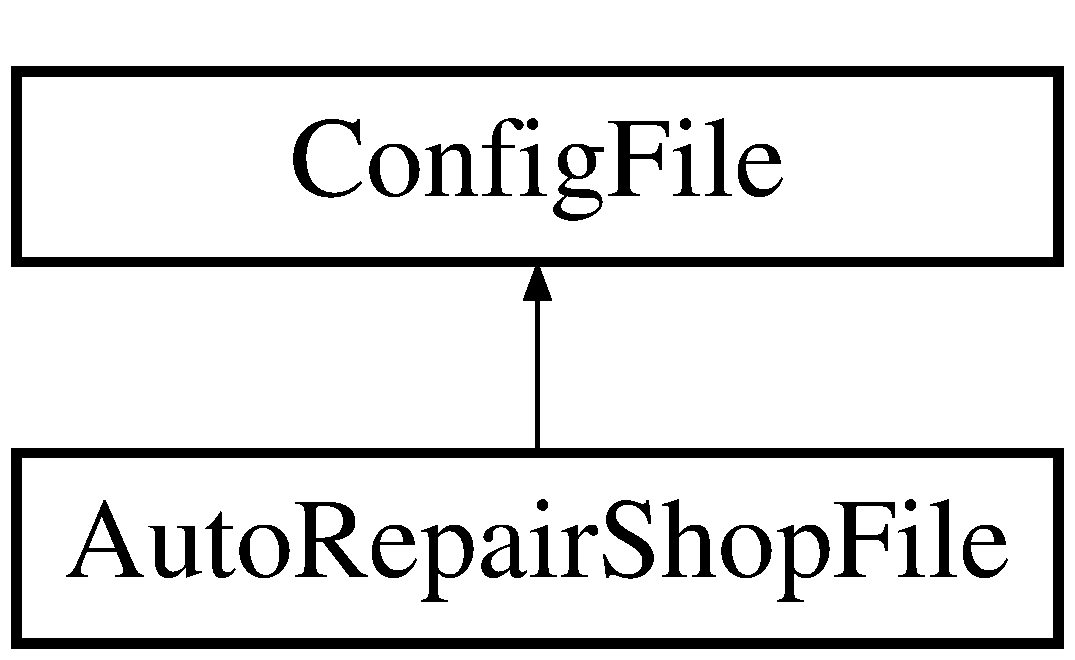
\includegraphics[height=2.000000cm]{class_auto_repair_shop_file}
\end{center}
\end{figure}
\subsection*{Public Member Functions}
\begin{DoxyCompactItemize}
\item 
\hypertarget{class_auto_repair_shop_file_a4b145da740e34dab9699072e5fb2bdb2}{}{\bfseries Auto\+Repair\+Shop\+File} (string \&filename)\label{class_auto_repair_shop_file_a4b145da740e34dab9699072e5fb2bdb2}

\item 
\hypertarget{class_auto_repair_shop_file_a5a695e232fcd555e0b735334ed4311d6}{}bool \hyperlink{class_auto_repair_shop_file_a5a695e232fcd555e0b735334ed4311d6}{save\+Data} (\hyperlink{class_auto_repair_shop}{Auto\+Repair\+Shop} \&repair\+Shop, string \&vehicles\+Filename, string \&clients\+Filename, string \&employees\+File\+Name, bool overwrite=false)\label{class_auto_repair_shop_file_a5a695e232fcd555e0b735334ed4311d6}

\begin{DoxyCompactList}\small\item\em saves the file data \end{DoxyCompactList}\item 
\hypertarget{class_auto_repair_shop_file_a52b87c845d50b6c8a8e9374cdeb1101a}{}\hyperlink{class_auto_repair_shop}{Auto\+Repair\+Shop} \hyperlink{class_auto_repair_shop_file_a52b87c845d50b6c8a8e9374cdeb1101a}{load\+Data} ()\label{class_auto_repair_shop_file_a52b87c845d50b6c8a8e9374cdeb1101a}

\begin{DoxyCompactList}\small\item\em loads data from the file, creating an \hyperlink{class_auto_repair_shop}{Auto\+Repair\+Shop} \end{DoxyCompactList}\end{DoxyCompactItemize}
\subsection*{Additional Inherited Members}


\subsection{Detailed Description}
contains the name of the vehiclesfile, clientsfile and employeesfile and the name of the Auto Repair Shop 

The documentation for this class was generated from the following files\+:\begin{DoxyCompactItemize}
\item 
Config\+File.\+h\item 
Config\+File.\+cpp\end{DoxyCompactItemize}

\hypertarget{class_config_file_1_1_bad_file_exception}{}\section{Config\+File\+:\+:Bad\+File\+Exception Class Reference}
\label{class_config_file_1_1_bad_file_exception}\index{Config\+File\+::\+Bad\+File\+Exception@{Config\+File\+::\+Bad\+File\+Exception}}


{\ttfamily \#include $<$Config\+File.\+h$>$}

Inheritance diagram for Config\+File\+:\+:Bad\+File\+Exception\+:\begin{figure}[H]
\begin{center}
\leavevmode
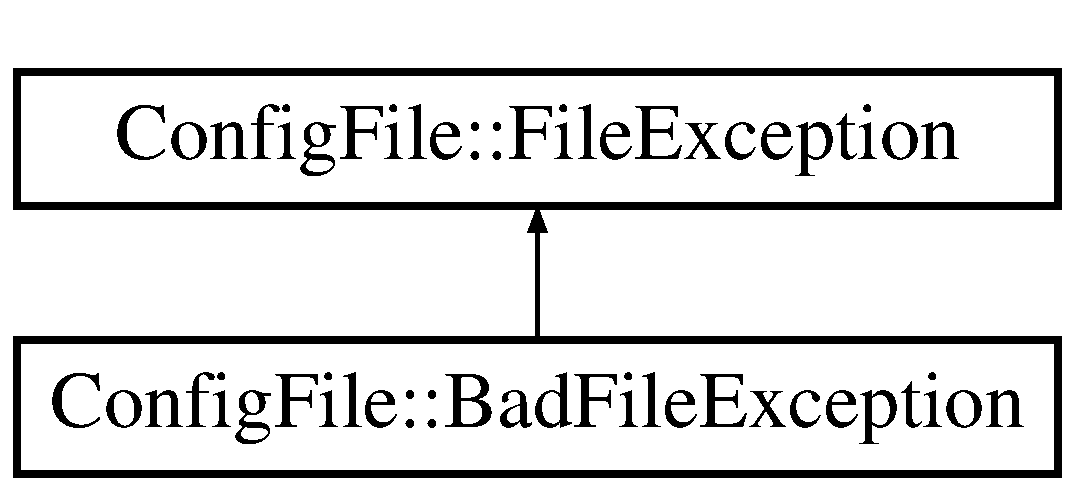
\includegraphics[height=2.000000cm]{class_config_file_1_1_bad_file_exception}
\end{center}
\end{figure}
\subsection*{Public Member Functions}
\begin{DoxyCompactItemize}
\item 
\hypertarget{class_config_file_1_1_bad_file_exception_a890ccce3543b355a3b514790e4218521}{}{\bfseries Bad\+File\+Exception} (string \&filename)\label{class_config_file_1_1_bad_file_exception_a890ccce3543b355a3b514790e4218521}

\item 
\hypertarget{class_config_file_1_1_bad_file_exception_a8f55fca6a89e4b32062abb2254b26155}{}void {\bfseries show\+Error\+Message} () const \label{class_config_file_1_1_bad_file_exception_a8f55fca6a89e4b32062abb2254b26155}

\end{DoxyCompactItemize}
\subsection*{Additional Inherited Members}


\subsection{Detailed Description}

\begin{DoxyExceptions}{Exceptions}
{\em \hyperlink{class_config_file_1_1_bad_file_exception}{Bad\+File\+Exception}} & exception to throw when the file has the wrong format \\
\hline
\end{DoxyExceptions}


The documentation for this class was generated from the following file\+:\begin{DoxyCompactItemize}
\item 
Config\+File.\+h\end{DoxyCompactItemize}

\hypertarget{class_bus}{}\section{Bus Class Reference}
\label{class_bus}\index{Bus@{Bus}}
Inheritance diagram for Bus\+:\begin{figure}[H]
\begin{center}
\leavevmode
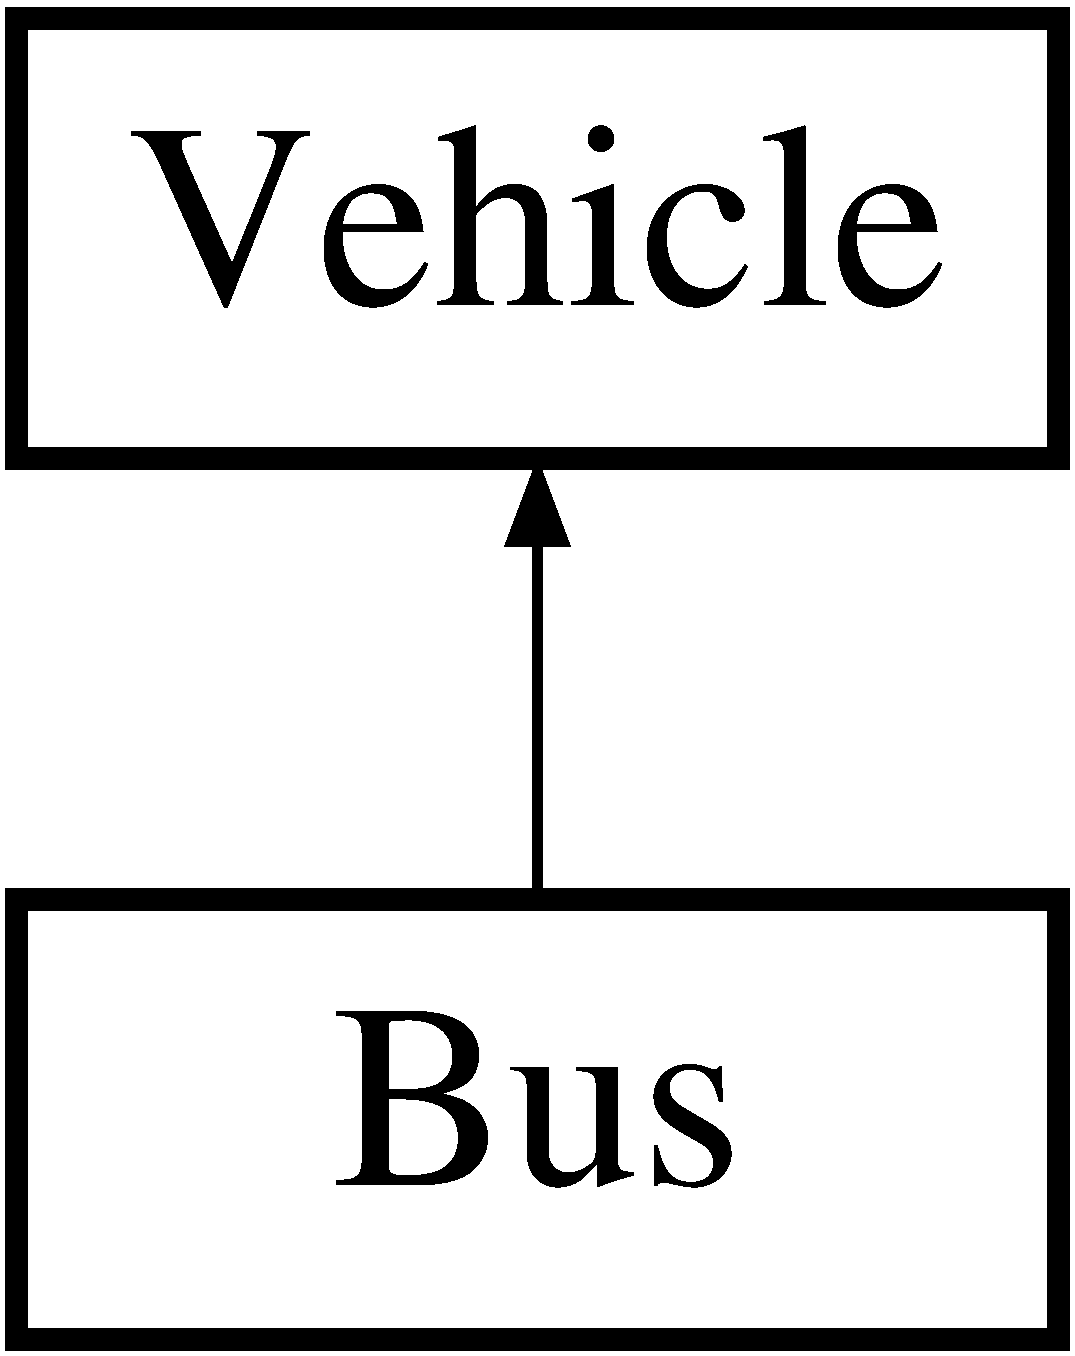
\includegraphics[height=2.000000cm]{class_bus}
\end{center}
\end{figure}
\subsection*{Public Member Functions}
\begin{DoxyCompactItemize}
\item 
\hypertarget{class_bus_adfb5b76cdad7c915cebf59b1670091ff}{}{\bfseries Bus} (string manufacturer, string model, string license\+Plate, int num\+Sitting\+Spots, int num\+Standing\+Spots)\label{class_bus_adfb5b76cdad7c915cebf59b1670091ff}

\item 
\hypertarget{class_bus_a272be09e059cd47be6793eaa4e853e0d}{}{\bfseries Bus} (istream \&in)\label{class_bus_a272be09e059cd47be6793eaa4e853e0d}

\item 
\hypertarget{class_bus_adc766f7d78116640cc5aeb52e22ae143}{}int {\bfseries class\+Identifier} ()\label{class_bus_adc766f7d78116640cc5aeb52e22ae143}

\item 
\hypertarget{class_bus_adf58347d7a8ae2a05548f5d5eef8b5dd}{}void {\bfseries save\+Object\+Info} (ostream \&out)\label{class_bus_adf58347d7a8ae2a05548f5d5eef8b5dd}

\item 
\hypertarget{class_bus_a5713a725a5c73412c2686d6bba61c9a4}{}void {\bfseries print\+Object\+Info} () const \label{class_bus_a5713a725a5c73412c2686d6bba61c9a4}

\end{DoxyCompactItemize}


The documentation for this class was generated from the following files\+:\begin{DoxyCompactItemize}
\item 
Vehicle.\+h\item 
Vehicle.\+cpp\end{DoxyCompactItemize}

\hypertarget{class_car_wash}{}\section{Car\+Wash Class Reference}
\label{class_car_wash}\index{Car\+Wash@{Car\+Wash}}
Inheritance diagram for Car\+Wash\+:\begin{figure}[H]
\begin{center}
\leavevmode
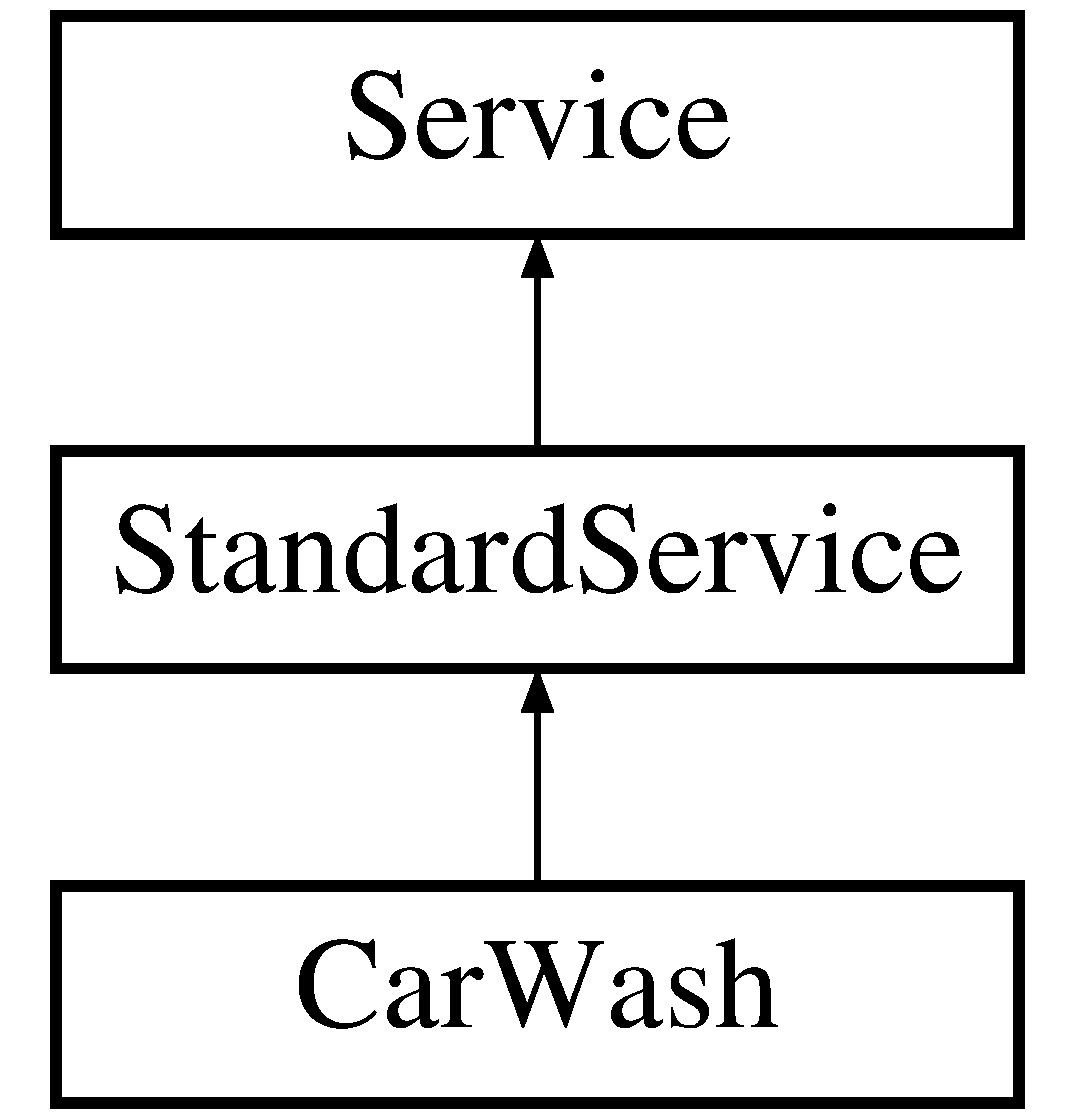
\includegraphics[height=3.000000cm]{class_car_wash}
\end{center}
\end{figure}
\subsection*{Public Member Functions}
\begin{DoxyCompactItemize}
\item 
\hypertarget{class_car_wash_a0e62c97aa6ea66728c35b81a97134f41}{}{\bfseries Car\+Wash} (\hyperlink{struct_date}{Date} starting\+Date)\label{class_car_wash_a0e62c97aa6ea66728c35b81a97134f41}

\item 
\hypertarget{class_car_wash_a4b5fa2957227df1358df80fe38443635}{}{\bfseries Car\+Wash} (istream \&in)\label{class_car_wash_a4b5fa2957227df1358df80fe38443635}

\item 
\hypertarget{class_car_wash_a0cdc63c1e52c987640b11f6a1351dc46}{}int {\bfseries class\+Identifier} ()\label{class_car_wash_a0cdc63c1e52c987640b11f6a1351dc46}

\item 
\hypertarget{class_car_wash_a3bda9ff2a0335b9da7116286c65cb05f}{}void {\bfseries save\+Object\+Info} (ostream \&out)\label{class_car_wash_a3bda9ff2a0335b9da7116286c65cb05f}

\item 
\hypertarget{class_car_wash_ade6abea7ff6b2e733811d05e53903bf0}{}float {\bfseries get\+Price} () const \label{class_car_wash_ade6abea7ff6b2e733811d05e53903bf0}

\item 
\hypertarget{class_car_wash_a8ab92c44fbafe9ccadc8714aa580cece}{}int {\bfseries get\+Duration} () const \label{class_car_wash_a8ab92c44fbafe9ccadc8714aa580cece}

\item 
\hypertarget{class_car_wash_a0ff92bfd45f847986468b61ad3b1abd2}{}const string \& {\bfseries get\+Description} () const \label{class_car_wash_a0ff92bfd45f847986468b61ad3b1abd2}

\end{DoxyCompactItemize}
\subsection*{Additional Inherited Members}


The documentation for this class was generated from the following files\+:\begin{DoxyCompactItemize}
\item 
Service.\+h\item 
Service.\+cpp\end{DoxyCompactItemize}

\hypertarget{class_client}{}\section{Client Class Reference}
\label{class_client}\index{Client@{Client}}


subclass of \hyperlink{class_person}{Person}, someone with cars on the Auto Repair Shop  




{\ttfamily \#include $<$Auto\+Repair\+Shop.\+h$>$}

Inheritance diagram for Client\+:\begin{figure}[H]
\begin{center}
\leavevmode
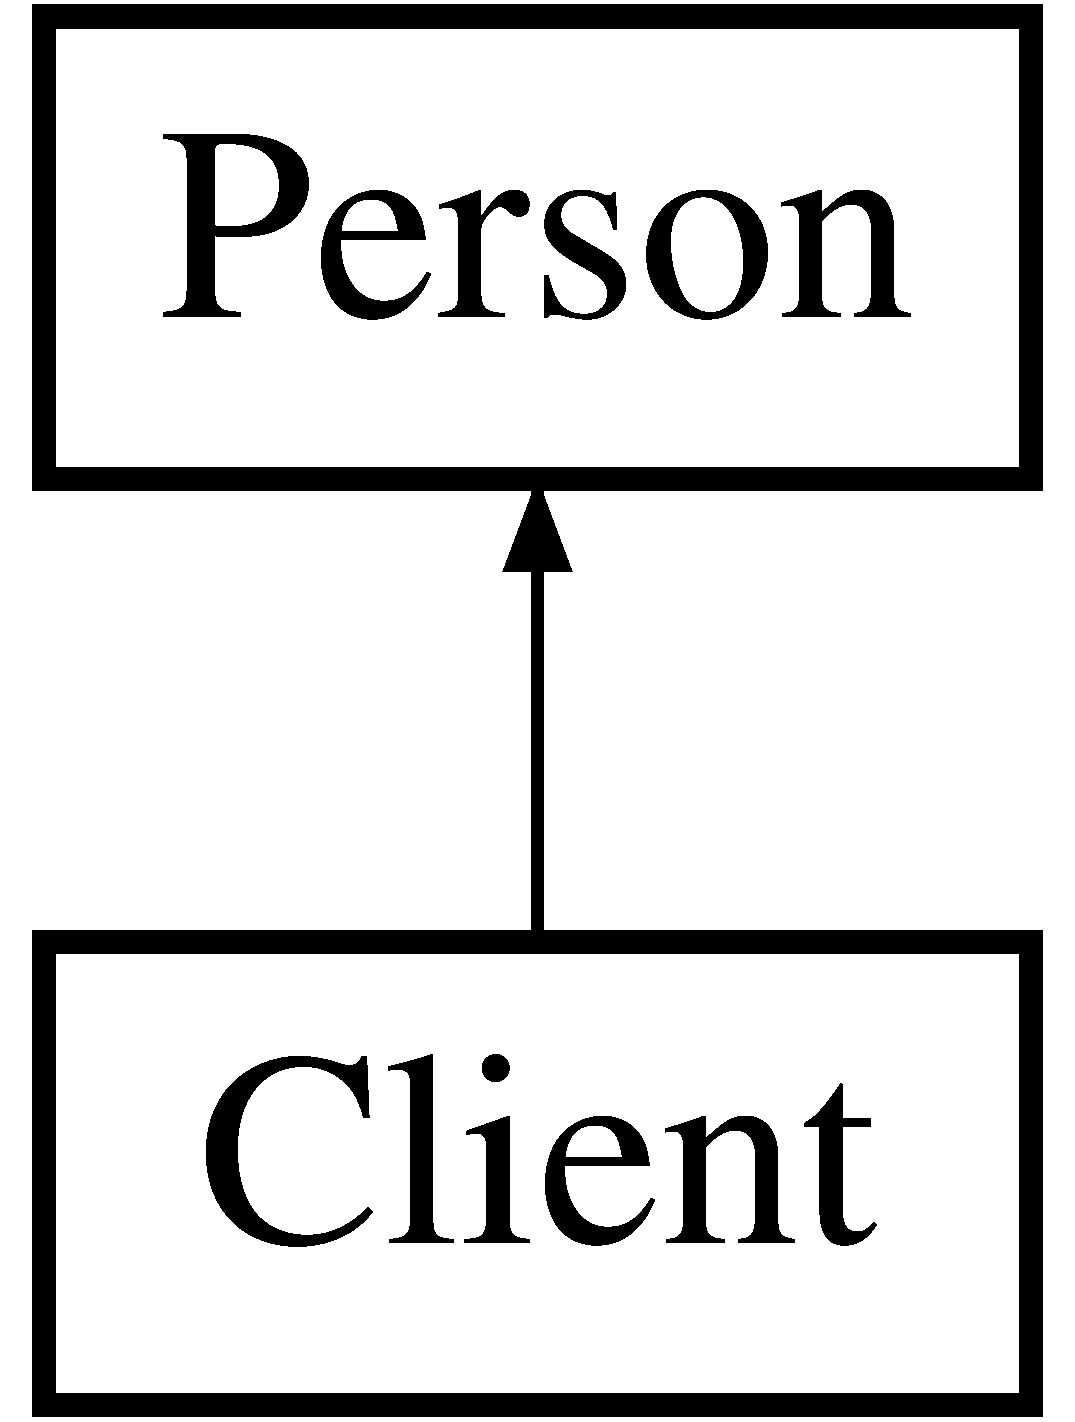
\includegraphics[height=2.000000cm]{class_client}
\end{center}
\end{figure}
\subsection*{Public Member Functions}
\begin{DoxyCompactItemize}
\item 
\hypertarget{class_client_a62ec00483394e1de13111094b221921d}{}\hyperlink{class_client_a62ec00483394e1de13111094b221921d}{Client} (string name)\label{class_client_a62ec00483394e1de13111094b221921d}

\begin{DoxyCompactList}\small\item\em creates an object of \hyperlink{class_client}{Client} class \end{DoxyCompactList}\item 
\hyperlink{class_client_aae5506d2aa6e4486f8e393b75ff5b5f4}{Client} (istream \&in, string name, vector$<$ string $>$ \&license\+Plates)
\begin{DoxyCompactList}\small\item\em reads an object of \hyperlink{class_client}{Client} class from a stream \end{DoxyCompactList}\item 
\hypertarget{class_client_a774e8af1c055d52dfe8a1db0847332d0}{}void \hyperlink{class_client_a774e8af1c055d52dfe8a1db0847332d0}{print\+Object\+Info} () const \label{class_client_a774e8af1c055d52dfe8a1db0847332d0}

\begin{DoxyCompactList}\small\item\em prints the objects\textquotesingle{} info to std\+::cout \end{DoxyCompactList}\item 
\hypertarget{class_client_aef483ed374ceca699aa17bc90fe82f68}{}void \hyperlink{class_client_aef483ed374ceca699aa17bc90fe82f68}{print\+Services} () const \label{class_client_aef483ed374ceca699aa17bc90fe82f68}

\begin{DoxyCompactList}\small\item\em prints to std\+::cout all services made on the client\textquotesingle{}s car \end{DoxyCompactList}\end{DoxyCompactItemize}
\subsection*{Additional Inherited Members}


\subsection{Detailed Description}
subclass of \hyperlink{class_person}{Person}, someone with cars on the Auto Repair Shop 

\subsection{Constructor \& Destructor Documentation}
\hypertarget{class_client_aae5506d2aa6e4486f8e393b75ff5b5f4}{}\index{Client@{Client}!Client@{Client}}
\index{Client@{Client}!Client@{Client}}
\subsubsection[{Client(istream \&in, string name, vector$<$ string $>$ \&license\+Plates)}]{\setlength{\rightskip}{0pt plus 5cm}Client\+::\+Client (
\begin{DoxyParamCaption}
\item[{istream \&}]{in, }
\item[{string}]{name, }
\item[{vector$<$ string $>$ \&}]{license\+Plates}
\end{DoxyParamCaption}
)\hspace{0.3cm}{\ttfamily [inline]}}\label{class_client_aae5506d2aa6e4486f8e393b75ff5b5f4}


reads an object of \hyperlink{class_client}{Client} class from a stream 


\begin{DoxyParams}[1]{Parameters}
\mbox{\tt out}  & {\em license\+Plates} & returns the license plates of all vehicles owned by \hyperlink{class_client}{Client} \\
\hline
\end{DoxyParams}


The documentation for this class was generated from the following files\+:\begin{DoxyCompactItemize}
\item 
Auto\+Repair\+Shop.\+h\item 
Auto\+Repair\+Shop.\+cpp\end{DoxyCompactItemize}

\hypertarget{class_clients_file}{}\section{Clients\+File Class Reference}
\label{class_clients_file}\index{Clients\+File@{Clients\+File}}


contains the info of all the clients of the Auto Repair Shop  




{\ttfamily \#include $<$Config\+File.\+h$>$}

Inheritance diagram for Clients\+File\+:\begin{figure}[H]
\begin{center}
\leavevmode
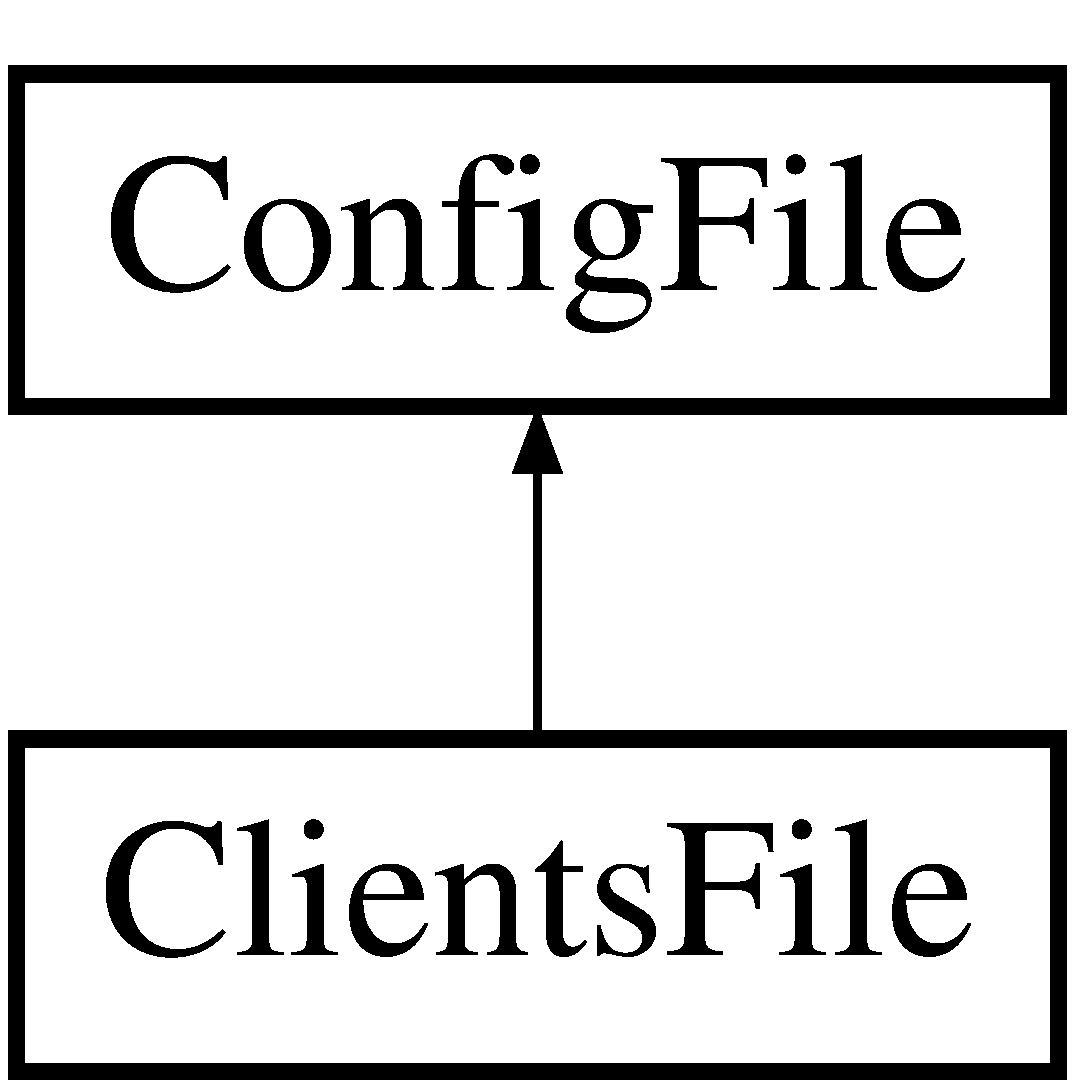
\includegraphics[height=2.000000cm]{class_clients_file}
\end{center}
\end{figure}
\subsection*{Public Member Functions}
\begin{DoxyCompactItemize}
\item 
\hypertarget{class_clients_file_a193a5c33a221b9a7a240c8e21325f5bc}{}{\bfseries Clients\+File} (string \&filename)\label{class_clients_file_a193a5c33a221b9a7a240c8e21325f5bc}

\item 
\hypertarget{class_clients_file_a208a3388f95c5b181708d82f24f73807}{}\hyperlink{class_client}{Client} \hyperlink{class_clients_file_a208a3388f95c5b181708d82f24f73807}{create\+Client\+Object} (istream \&in, string name, vector$<$ string $>$ license\+Plates, \hyperlink{class_auto_repair_shop}{Auto\+Repair\+Shop} \&repair\+Shop)\label{class_clients_file_a208a3388f95c5b181708d82f24f73807}

\begin{DoxyCompactList}\small\item\em creates and returns a client, adding all vehicles with license plates on the license\+Plates vector \end{DoxyCompactList}\item 
\hypertarget{class_clients_file_a036db9670a49d65576c9b16f6c97b225}{}bool \hyperlink{class_clients_file_a036db9670a49d65576c9b16f6c97b225}{save\+Data} (\hyperlink{class_auto_repair_shop}{Auto\+Repair\+Shop} \&repair\+Shop, bool overwrite=false)\label{class_clients_file_a036db9670a49d65576c9b16f6c97b225}

\begin{DoxyCompactList}\small\item\em saves the file data \end{DoxyCompactList}\item 
bool \hyperlink{class_clients_file_a503c04b5e98494318abf2a26a0348de9}{load\+Data} (\hyperlink{class_auto_repair_shop}{Auto\+Repair\+Shop} \&repair\+Shop)
\begin{DoxyCompactList}\small\item\em loads data from the file \end{DoxyCompactList}\end{DoxyCompactItemize}
\subsection*{Additional Inherited Members}


\subsection{Detailed Description}
contains the info of all the clients of the Auto Repair Shop 

contains the info of all the Auto Repair Shop\textquotesingle{}s employees 

\subsection{Member Function Documentation}
\hypertarget{class_clients_file_a503c04b5e98494318abf2a26a0348de9}{}\index{Clients\+File@{Clients\+File}!load\+Data@{load\+Data}}
\index{load\+Data@{load\+Data}!Clients\+File@{Clients\+File}}
\subsubsection[{load\+Data(\+Auto\+Repair\+Shop \&repair\+Shop)}]{\setlength{\rightskip}{0pt plus 5cm}bool Clients\+File\+::load\+Data (
\begin{DoxyParamCaption}
\item[{{\bf Auto\+Repair\+Shop} \&}]{repair\+Shop}
\end{DoxyParamCaption}
)}\label{class_clients_file_a503c04b5e98494318abf2a26a0348de9}


loads data from the file 

\begin{DoxyReturn}{Returns}
false if the file doesn\textquotesingle{}t exist 
\end{DoxyReturn}


The documentation for this class was generated from the following files\+:\begin{DoxyCompactItemize}
\item 
Config\+File.\+h\item 
Config\+File.\+cpp\end{DoxyCompactItemize}

\hypertarget{class_config_file}{}\section{Config\+File Class Reference}
\label{class_config_file}\index{Config\+File@{Config\+File}}


superclass to all types of file Keeps their common behaviour  




{\ttfamily \#include $<$Config\+File.\+h$>$}

Inheritance diagram for Config\+File\+:\begin{figure}[H]
\begin{center}
\leavevmode
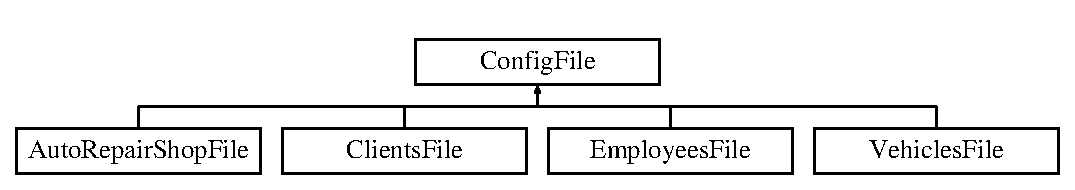
\includegraphics[height=2.000000cm]{class_config_file}
\end{center}
\end{figure}
\subsection*{Classes}
\begin{DoxyCompactItemize}
\item 
class \hyperlink{class_config_file_1_1_bad_file_exception}{Bad\+File\+Exception}
\item 
class \hyperlink{class_config_file_1_1_empty_file_exception}{Empty\+File\+Exception}
\item 
class \hyperlink{class_config_file_1_1_file_exception}{File\+Exception}
\item 
class \hyperlink{class_config_file_1_1_inexistent_file_exception}{Inexistent\+File\+Exception}
\end{DoxyCompactItemize}
\subsection*{Public Member Functions}
\begin{DoxyCompactItemize}
\item 
\hypertarget{class_config_file_a0f9b83c045bfe0ef78d008fa26d893c4}{}\hyperlink{class_config_file_a0f9b83c045bfe0ef78d008fa26d893c4}{Config\+File} (string \&filename)\label{class_config_file_a0f9b83c045bfe0ef78d008fa26d893c4}

\begin{DoxyCompactList}\small\item\em creates a \hyperlink{class_config_file}{Config\+File} object \end{DoxyCompactList}\item 
\hypertarget{class_config_file_a0a3050a665cd0c0d9eece2ba4690a43e}{}void \hyperlink{class_config_file_a0a3050a665cd0c0d9eece2ba4690a43e}{create\+File} (string \&filename)\label{class_config_file_a0a3050a665cd0c0d9eece2ba4690a43e}

\begin{DoxyCompactList}\small\item\em creates a file with given filename \end{DoxyCompactList}\item 
bool \hyperlink{class_config_file_a31ca66b91dfa8d9a7f1b37a01e57de3f}{exists\+File} (string \&filename)
\end{DoxyCompactItemize}
\subsection*{Protected Attributes}
\begin{DoxyCompactItemize}
\item 
\hypertarget{class_config_file_a89923d5ab6a13a1ceb0d10a6188765d3}{}string {\bfseries filename}\label{class_config_file_a89923d5ab6a13a1ceb0d10a6188765d3}

\end{DoxyCompactItemize}


\subsection{Detailed Description}
superclass to all types of file Keeps their common behaviour 

\subsection{Member Function Documentation}
\hypertarget{class_config_file_a31ca66b91dfa8d9a7f1b37a01e57de3f}{}\index{Config\+File@{Config\+File}!exists\+File@{exists\+File}}
\index{exists\+File@{exists\+File}!Config\+File@{Config\+File}}
\subsubsection[{exists\+File(string \&filename)}]{\setlength{\rightskip}{0pt plus 5cm}bool Config\+File\+::exists\+File (
\begin{DoxyParamCaption}
\item[{string \&}]{filename}
\end{DoxyParamCaption}
)}\label{class_config_file_a31ca66b91dfa8d9a7f1b37a01e57de3f}
\begin{DoxyReturn}{Returns}
true if a file with the given filename exists 

false if it doesn\textquotesingle{}t exist 
\end{DoxyReturn}


The documentation for this class was generated from the following files\+:\begin{DoxyCompactItemize}
\item 
Config\+File.\+h\item 
Config\+File.\+cpp\end{DoxyCompactItemize}

\hypertarget{struct_date}{}\section{Date Struct Reference}
\label{struct_date}\index{Date@{Date}}
\subsection*{Public Attributes}
\begin{DoxyCompactItemize}
\item 
\hypertarget{struct_date_a5b192adcabf2b2871e3f0b76c1ec1601}{}int {\bfseries day}\label{struct_date_a5b192adcabf2b2871e3f0b76c1ec1601}

\item 
\hypertarget{struct_date_a533843e07c6ac8d19fee9b16f5336ba2}{}int {\bfseries month}\label{struct_date_a533843e07c6ac8d19fee9b16f5336ba2}

\item 
\hypertarget{struct_date_a3eeced2ed56bc95d56782b9e738db8ea}{}int {\bfseries year}\label{struct_date_a3eeced2ed56bc95d56782b9e738db8ea}

\end{DoxyCompactItemize}


The documentation for this struct was generated from the following file\+:\begin{DoxyCompactItemize}
\item 
Service.\+h\end{DoxyCompactItemize}

\hypertarget{class_employee}{}\section{Employee Class Reference}
\label{class_employee}\index{Employee@{Employee}}


subclass of \hyperlink{class_person}{Person}, responsible by cars on the Auto Repair Shop  




{\ttfamily \#include $<$Auto\+Repair\+Shop.\+h$>$}

Inheritance diagram for Employee\+:\begin{figure}[H]
\begin{center}
\leavevmode
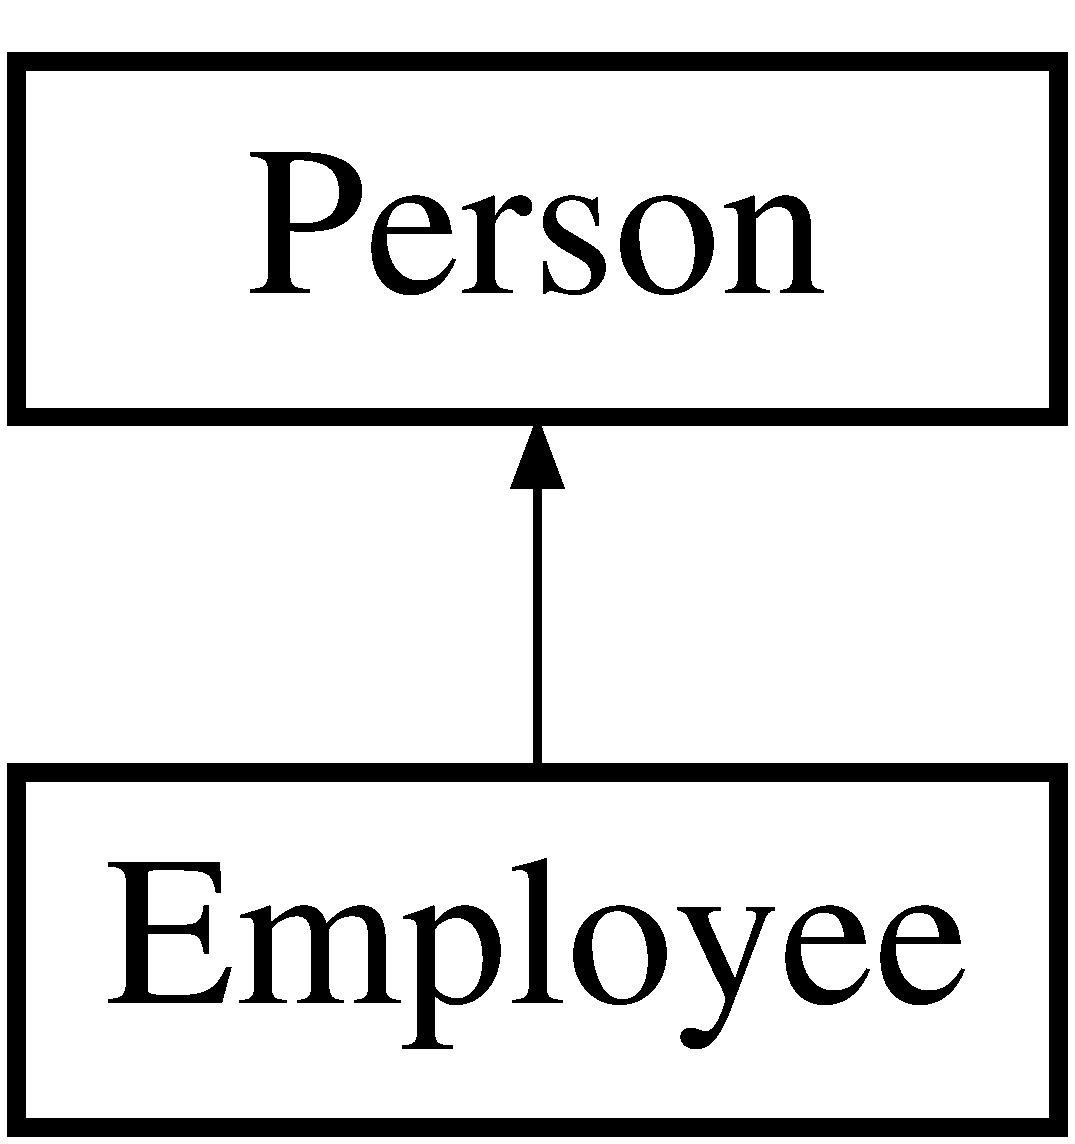
\includegraphics[height=2.000000cm]{class_employee}
\end{center}
\end{figure}
\subsection*{Public Member Functions}
\begin{DoxyCompactItemize}
\item 
\hypertarget{class_employee_a7ee153c7da11b23eb6bb7649fbb5797b}{}\hyperlink{class_employee_a7ee153c7da11b23eb6bb7649fbb5797b}{Employee} (string name)\label{class_employee_a7ee153c7da11b23eb6bb7649fbb5797b}

\begin{DoxyCompactList}\small\item\em creates an object of \hyperlink{class_employee}{Employee} class \end{DoxyCompactList}\item 
\hyperlink{class_employee_a494ea647c0cbeae14352add1e2e9dbf8}{Employee} (istream \&in, string name, vector$<$ string $>$ \&license\+Plates)
\begin{DoxyCompactList}\small\item\em reads an object of \hyperlink{class_employee}{Employee} class from a stream \end{DoxyCompactList}\item 
\hypertarget{class_employee_a1d85f1648beb9ba8921463948fd37273}{}void \hyperlink{class_employee_a1d85f1648beb9ba8921463948fd37273}{print\+Object\+Info} () const \label{class_employee_a1d85f1648beb9ba8921463948fd37273}

\begin{DoxyCompactList}\small\item\em prints the objects\textquotesingle{} info to std\+::cout \end{DoxyCompactList}\end{DoxyCompactItemize}
\subsection*{Additional Inherited Members}


\subsection{Detailed Description}
subclass of \hyperlink{class_person}{Person}, responsible by cars on the Auto Repair Shop 

\subsection{Constructor \& Destructor Documentation}
\hypertarget{class_employee_a494ea647c0cbeae14352add1e2e9dbf8}{}\index{Employee@{Employee}!Employee@{Employee}}
\index{Employee@{Employee}!Employee@{Employee}}
\subsubsection[{Employee(istream \&in, string name, vector$<$ string $>$ \&license\+Plates)}]{\setlength{\rightskip}{0pt plus 5cm}Employee\+::\+Employee (
\begin{DoxyParamCaption}
\item[{istream \&}]{in, }
\item[{string}]{name, }
\item[{vector$<$ string $>$ \&}]{license\+Plates}
\end{DoxyParamCaption}
)\hspace{0.3cm}{\ttfamily [inline]}}\label{class_employee_a494ea647c0cbeae14352add1e2e9dbf8}


reads an object of \hyperlink{class_employee}{Employee} class from a stream 


\begin{DoxyParams}[1]{Parameters}
\mbox{\tt out}  & {\em license\+Plates} & returns the license plates of all vehicles assigned to \hyperlink{class_employee}{Employee} \\
\hline
\end{DoxyParams}


The documentation for this class was generated from the following files\+:\begin{DoxyCompactItemize}
\item 
Auto\+Repair\+Shop.\+h\item 
Auto\+Repair\+Shop.\+cpp\end{DoxyCompactItemize}

\hypertarget{class_employees_file}{}\section{Employees\+File Class Reference}
\label{class_employees_file}\index{Employees\+File@{Employees\+File}}
Inheritance diagram for Employees\+File\+:\begin{figure}[H]
\begin{center}
\leavevmode
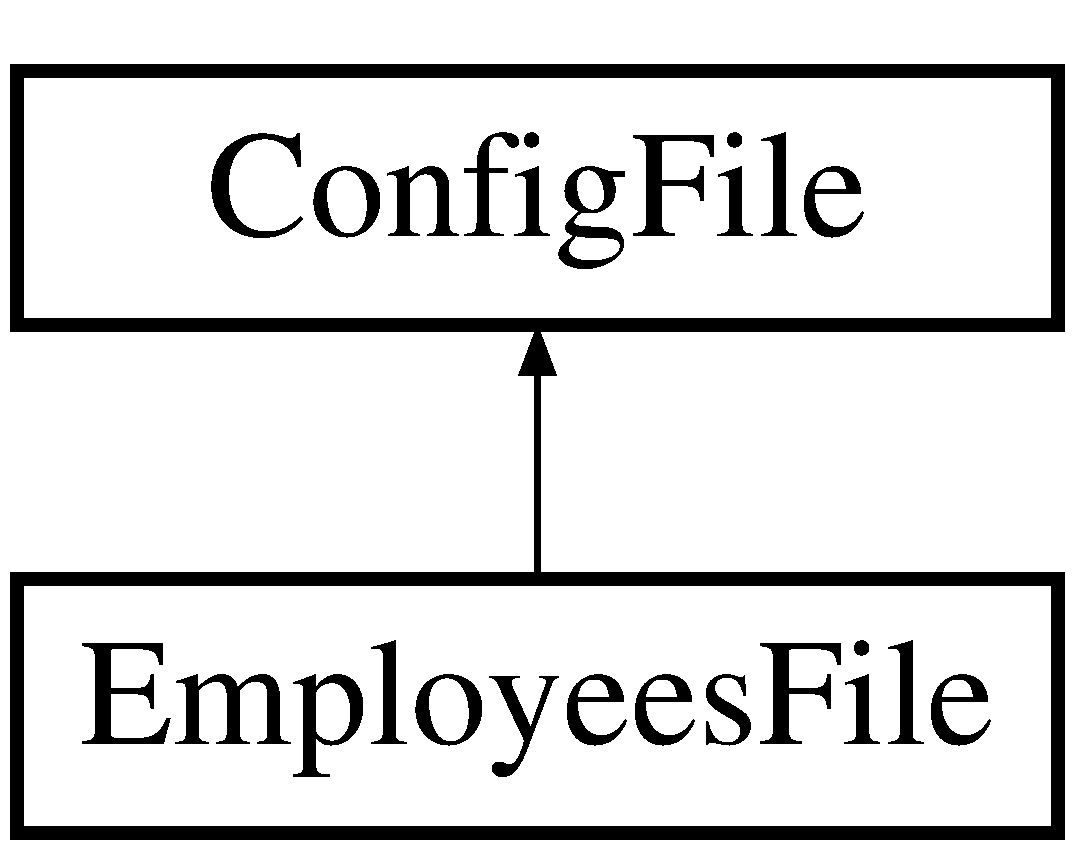
\includegraphics[height=2.000000cm]{class_employees_file}
\end{center}
\end{figure}
\subsection*{Public Member Functions}
\begin{DoxyCompactItemize}
\item 
\hypertarget{class_employees_file_a8f029a7de1acc27856a379813c4c03e0}{}{\bfseries Employees\+File} (string \&filename)\label{class_employees_file_a8f029a7de1acc27856a379813c4c03e0}

\item 
\hypertarget{class_employees_file_a4e36311279ed0aab10435eaac5126151}{}\hyperlink{class_employee}{Employee} \hyperlink{class_employees_file_a4e36311279ed0aab10435eaac5126151}{create\+Employee\+Object} (istream \&in, string name, vector$<$ string $>$ license\+Plates, \hyperlink{class_auto_repair_shop}{Auto\+Repair\+Shop} \&repair\+Shop)\label{class_employees_file_a4e36311279ed0aab10435eaac5126151}

\begin{DoxyCompactList}\small\item\em creates and returns an employee, adding all vehicles with license plates on the license\+Plates vector \end{DoxyCompactList}\item 
\hypertarget{class_employees_file_aa9b65666486f2657808953bf2d9492f4}{}bool \hyperlink{class_employees_file_aa9b65666486f2657808953bf2d9492f4}{save\+Data} (\hyperlink{class_auto_repair_shop}{Auto\+Repair\+Shop} \&repair\+Shop, bool overwrite=false)\label{class_employees_file_aa9b65666486f2657808953bf2d9492f4}

\begin{DoxyCompactList}\small\item\em saves the file data \end{DoxyCompactList}\item 
bool \hyperlink{class_employees_file_a016b7476237e69b8f08925e85a0cba30}{load\+Data} (\hyperlink{class_auto_repair_shop}{Auto\+Repair\+Shop} \&repair\+Shop)
\begin{DoxyCompactList}\small\item\em loads data from the file \end{DoxyCompactList}\end{DoxyCompactItemize}
\subsection*{Additional Inherited Members}


\subsection{Member Function Documentation}
\hypertarget{class_employees_file_a016b7476237e69b8f08925e85a0cba30}{}\index{Employees\+File@{Employees\+File}!load\+Data@{load\+Data}}
\index{load\+Data@{load\+Data}!Employees\+File@{Employees\+File}}
\subsubsection[{load\+Data(\+Auto\+Repair\+Shop \&repair\+Shop)}]{\setlength{\rightskip}{0pt plus 5cm}bool Employees\+File\+::load\+Data (
\begin{DoxyParamCaption}
\item[{{\bf Auto\+Repair\+Shop} \&}]{repair\+Shop}
\end{DoxyParamCaption}
)}\label{class_employees_file_a016b7476237e69b8f08925e85a0cba30}


loads data from the file 

\begin{DoxyReturn}{Returns}
false if the file doesn\textquotesingle{}t exist 
\end{DoxyReturn}


The documentation for this class was generated from the following files\+:\begin{DoxyCompactItemize}
\item 
Config\+File.\+h\item 
Config\+File.\+cpp\end{DoxyCompactItemize}

\hypertarget{class_config_file_1_1_empty_file_exception}{}\section{Config\+File\+:\+:Empty\+File\+Exception Class Reference}
\label{class_config_file_1_1_empty_file_exception}\index{Config\+File\+::\+Empty\+File\+Exception@{Config\+File\+::\+Empty\+File\+Exception}}


{\ttfamily \#include $<$Config\+File.\+h$>$}



\subsection{Detailed Description}

\begin{DoxyExceptions}{Exceptions}
{\em \hyperlink{class_config_file_1_1_inexistent_file_exception}{Inexistent\+File\+Exception}} & exception to throw when the file doesn\textquotesingle{}t exists \\
\hline
\end{DoxyExceptions}


The documentation for this class was generated from the following file\+:\begin{DoxyCompactItemize}
\item 
Config\+File.\+h\end{DoxyCompactItemize}

\hypertarget{class_config_file_1_1_file_exception}{}\section{Config\+File\+:\+:File\+Exception Class Reference}
\label{class_config_file_1_1_file_exception}\index{Config\+File\+::\+File\+Exception@{Config\+File\+::\+File\+Exception}}


{\ttfamily \#include $<$Config\+File.\+h$>$}

Inheritance diagram for Config\+File\+:\+:File\+Exception\+:\begin{figure}[H]
\begin{center}
\leavevmode
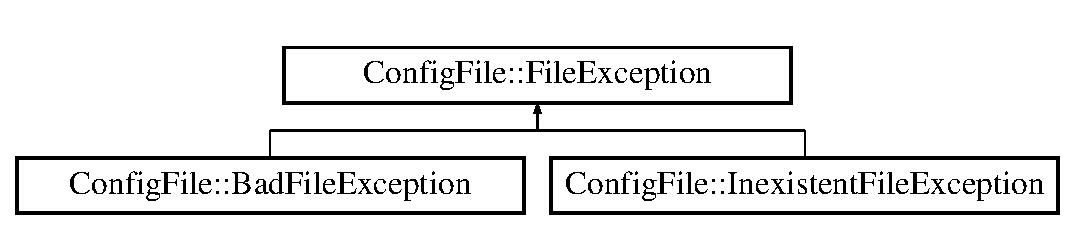
\includegraphics[height=2.000000cm]{class_config_file_1_1_file_exception}
\end{center}
\end{figure}
\subsection*{Public Member Functions}
\begin{DoxyCompactItemize}
\item 
\hypertarget{class_config_file_1_1_file_exception_ac0ef1dc6fab3adf968f4840659a7fd6e}{}{\bfseries File\+Exception} (string \&filename)\label{class_config_file_1_1_file_exception_ac0ef1dc6fab3adf968f4840659a7fd6e}

\item 
\hypertarget{class_config_file_1_1_file_exception_aec049b6e0245146d52f0feba60ccd12c}{}const string \& {\bfseries get\+Filename} () const \label{class_config_file_1_1_file_exception_aec049b6e0245146d52f0feba60ccd12c}

\item 
\hypertarget{class_config_file_1_1_file_exception_abda277ef553415617acf0253594af189}{}virtual void {\bfseries show\+Error\+Message} () const  =0\label{class_config_file_1_1_file_exception_abda277ef553415617acf0253594af189}

\end{DoxyCompactItemize}
\subsection*{Protected Attributes}
\begin{DoxyCompactItemize}
\item 
\hypertarget{class_config_file_1_1_file_exception_a1f1eda91b120d28cbeee5e0a5856a3f7}{}string {\bfseries filename}\label{class_config_file_1_1_file_exception_a1f1eda91b120d28cbeee5e0a5856a3f7}

\end{DoxyCompactItemize}


\subsection{Detailed Description}

\begin{DoxyExceptions}{Exceptions}
{\em \hyperlink{class_config_file_1_1_file_exception}{File\+Exception}} & superclass has the common behaviour of File-\/related exceptions \\
\hline
\end{DoxyExceptions}


The documentation for this class was generated from the following file\+:\begin{DoxyCompactItemize}
\item 
Config\+File.\+h\end{DoxyCompactItemize}

\hypertarget{class_config_file_1_1_inexistent_file_exception}{}\section{Config\+File\+:\+:Inexistent\+File\+Exception Class Reference}
\label{class_config_file_1_1_inexistent_file_exception}\index{Config\+File\+::\+Inexistent\+File\+Exception@{Config\+File\+::\+Inexistent\+File\+Exception}}


{\ttfamily \#include $<$Config\+File.\+h$>$}

Inheritance diagram for Config\+File\+:\+:Inexistent\+File\+Exception\+:\begin{figure}[H]
\begin{center}
\leavevmode
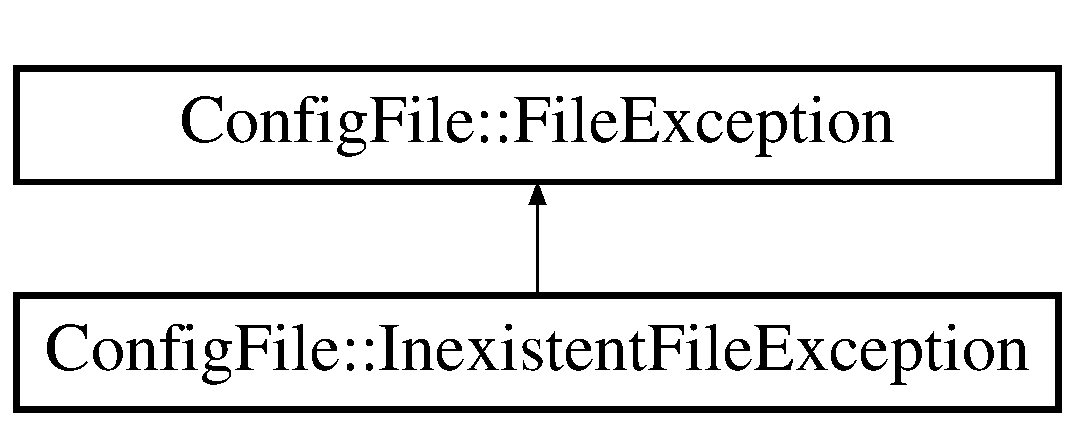
\includegraphics[height=2.000000cm]{class_config_file_1_1_inexistent_file_exception}
\end{center}
\end{figure}
\subsection*{Public Member Functions}
\begin{DoxyCompactItemize}
\item 
\hypertarget{class_config_file_1_1_inexistent_file_exception_a83a4ea384ce2811c689844b5b9bc83dd}{}{\bfseries Inexistent\+File\+Exception} (string \&filename)\label{class_config_file_1_1_inexistent_file_exception_a83a4ea384ce2811c689844b5b9bc83dd}

\item 
\hypertarget{class_config_file_1_1_inexistent_file_exception_a1ef632e719a76c22ffb10d5c402551c5}{}void {\bfseries show\+Error\+Message} () const \label{class_config_file_1_1_inexistent_file_exception_a1ef632e719a76c22ffb10d5c402551c5}

\end{DoxyCompactItemize}
\subsection*{Additional Inherited Members}


\subsection{Detailed Description}

\begin{DoxyExceptions}{Exceptions}
{\em \hyperlink{class_config_file_1_1_inexistent_file_exception}{Inexistent\+File\+Exception}} & exception to throw when the file doesn\textquotesingle{}t exists \\
\hline
\end{DoxyExceptions}


The documentation for this class was generated from the following file\+:\begin{DoxyCompactItemize}
\item 
Config\+File.\+h\end{DoxyCompactItemize}

\hypertarget{class_auto_repair_shop_1_1_inexistent_vehicle}{}\section{Auto\+Repair\+Shop\+:\+:Inexistent\+Vehicle Class Reference}
\label{class_auto_repair_shop_1_1_inexistent_vehicle}\index{Auto\+Repair\+Shop\+::\+Inexistent\+Vehicle@{Auto\+Repair\+Shop\+::\+Inexistent\+Vehicle}}


{\ttfamily \#include $<$Auto\+Repair\+Shop.\+h$>$}

\subsection*{Public Member Functions}
\begin{DoxyCompactItemize}
\item 
\hypertarget{class_auto_repair_shop_1_1_inexistent_vehicle_a0407499d2b9344073f5374a8a1e08bfb}{}{\bfseries Inexistent\+Vehicle} (string license\+Plate)\label{class_auto_repair_shop_1_1_inexistent_vehicle_a0407499d2b9344073f5374a8a1e08bfb}

\item 
\hypertarget{class_auto_repair_shop_1_1_inexistent_vehicle_ab663cb9d1dc102256af11334bd9dd042}{}void {\bfseries show\+Error\+Message} ()\label{class_auto_repair_shop_1_1_inexistent_vehicle_ab663cb9d1dc102256af11334bd9dd042}

\end{DoxyCompactItemize}


\subsection{Detailed Description}

\begin{DoxyExceptions}{Exceptions}
{\em \hyperlink{class_auto_repair_shop_1_1_inexistent_vehicle}{Inexistent\+Vehicle}} & exception to throw when \hyperlink{class_auto_repair_shop_afe7e5e9fdfb2c2e1e672eec1702999f4}{vehicle\+With\+License\+Plate()} doesn\textquotesingle{}t find any vehicle \\
\hline
\end{DoxyExceptions}


The documentation for this class was generated from the following file\+:\begin{DoxyCompactItemize}
\item 
Auto\+Repair\+Shop.\+h\end{DoxyCompactItemize}

\hypertarget{class_inspection}{}\section{Inspection Class Reference}
\label{class_inspection}\index{Inspection@{Inspection}}
Inheritance diagram for Inspection\+:\begin{figure}[H]
\begin{center}
\leavevmode
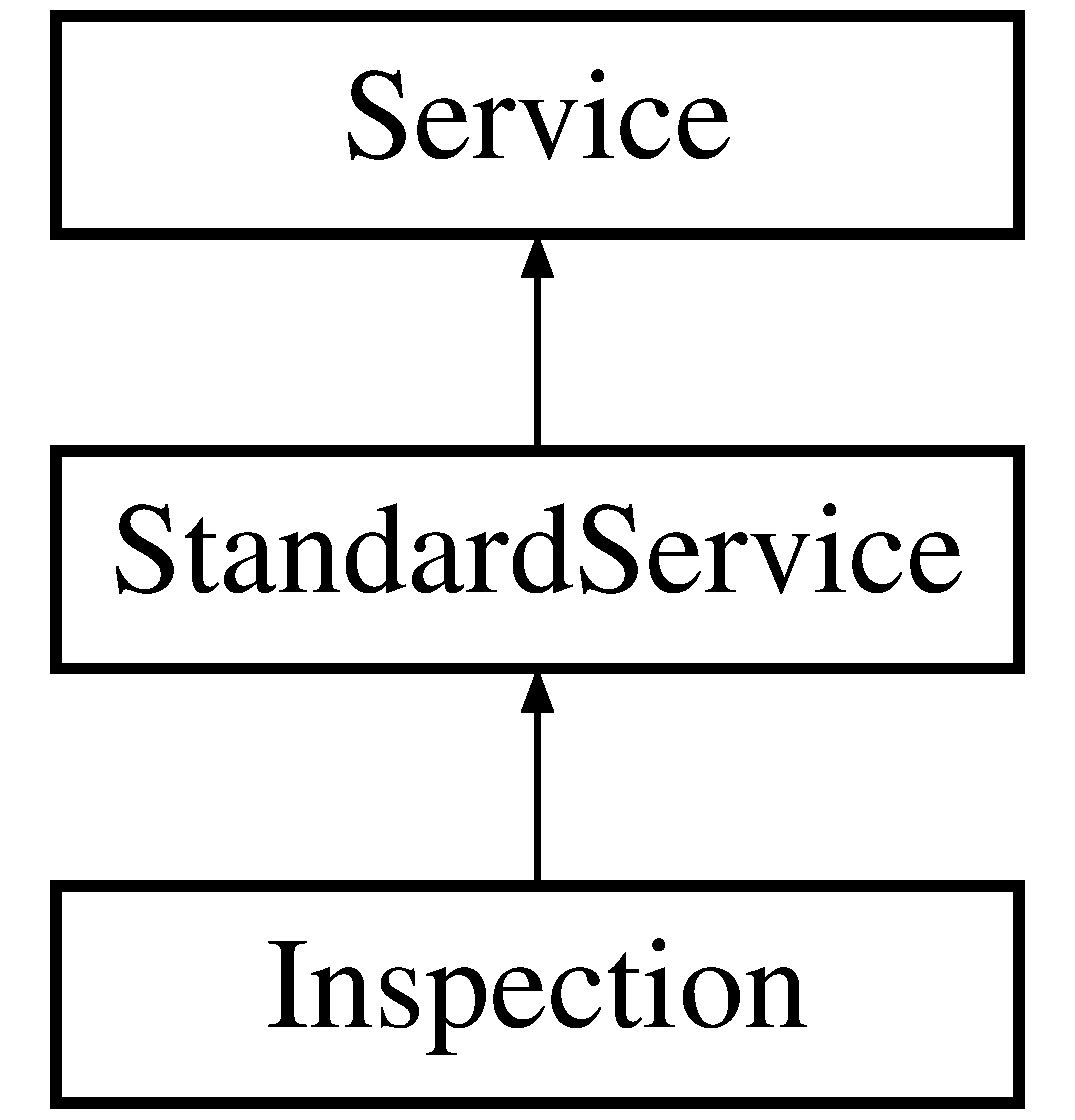
\includegraphics[height=3.000000cm]{class_inspection}
\end{center}
\end{figure}
\subsection*{Public Member Functions}
\begin{DoxyCompactItemize}
\item 
\hypertarget{class_inspection_a4197cde5b81c545a48c884b4db758c52}{}{\bfseries Inspection} (\hyperlink{struct_date}{Date} starting\+Date)\label{class_inspection_a4197cde5b81c545a48c884b4db758c52}

\item 
\hypertarget{class_inspection_abfeb16e2c97e6e19fd3647adf322c9f4}{}{\bfseries Inspection} (istream \&in)\label{class_inspection_abfeb16e2c97e6e19fd3647adf322c9f4}

\item 
\hypertarget{class_inspection_a0ad13e8e242dd41ad35f6713243f1730}{}int {\bfseries class\+Identifier} ()\label{class_inspection_a0ad13e8e242dd41ad35f6713243f1730}

\item 
\hypertarget{class_inspection_a17aad60b13f4ebff6db6081aa85e1b90}{}void {\bfseries save\+Object\+Info} (ostream \&out)\label{class_inspection_a17aad60b13f4ebff6db6081aa85e1b90}

\item 
\hypertarget{class_inspection_a3bad9f812251a99b7d2ffc5d0cf6d722}{}float {\bfseries get\+Price} () const \label{class_inspection_a3bad9f812251a99b7d2ffc5d0cf6d722}

\item 
\hypertarget{class_inspection_ad15f23a330708874ed5fe733418c0c7a}{}int {\bfseries get\+Duration} () const \label{class_inspection_ad15f23a330708874ed5fe733418c0c7a}

\item 
\hypertarget{class_inspection_a4abfb814dbf9a270c5dded4ef952d5c5}{}const string \& {\bfseries get\+Description} () const \label{class_inspection_a4abfb814dbf9a270c5dded4ef952d5c5}

\end{DoxyCompactItemize}
\subsection*{Additional Inherited Members}


The documentation for this class was generated from the following files\+:\begin{DoxyCompactItemize}
\item 
Service.\+h\item 
Service.\+cpp\end{DoxyCompactItemize}

\hypertarget{class_motorcycle}{}\section{Motorcycle Class Reference}
\label{class_motorcycle}\index{Motorcycle@{Motorcycle}}
Inheritance diagram for Motorcycle\+:\begin{figure}[H]
\begin{center}
\leavevmode
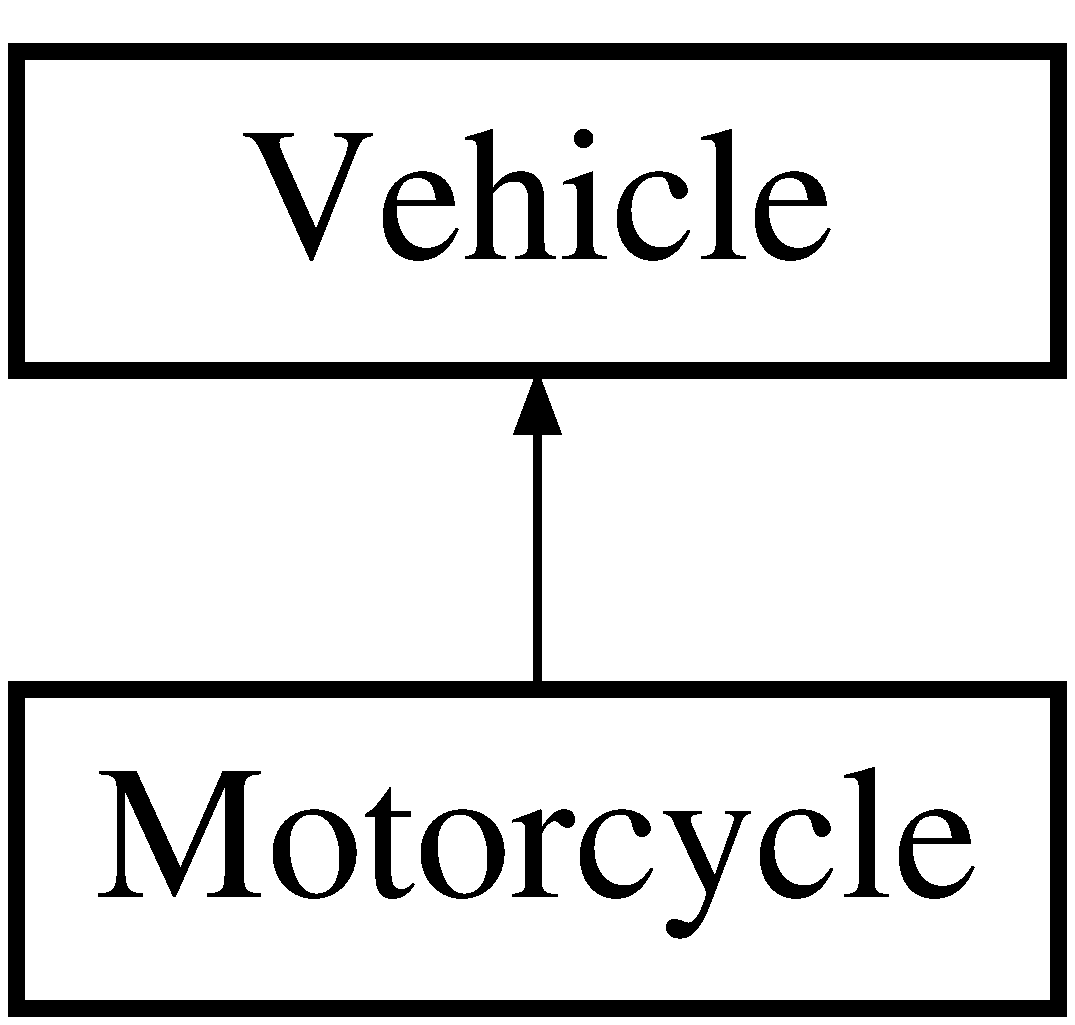
\includegraphics[height=2.000000cm]{class_motorcycle}
\end{center}
\end{figure}
\subsection*{Public Member Functions}
\begin{DoxyCompactItemize}
\item 
\hypertarget{class_motorcycle_abe8c77f57d12d47162ae04a571955491}{}{\bfseries Motorcycle} (string manufacturer, string model, string license\+Plate, string type)\label{class_motorcycle_abe8c77f57d12d47162ae04a571955491}

\item 
\hypertarget{class_motorcycle_a3a9d3b9f1584e736612fcfb6232fb4f9}{}{\bfseries Motorcycle} (istream \&in)\label{class_motorcycle_a3a9d3b9f1584e736612fcfb6232fb4f9}

\item 
\hypertarget{class_motorcycle_a85a9d67156047b9b416d7fb263bf4917}{}int {\bfseries class\+Identifier} ()\label{class_motorcycle_a85a9d67156047b9b416d7fb263bf4917}

\item 
\hypertarget{class_motorcycle_a52febae0045ecd03806b9e59ac98d3af}{}void {\bfseries save\+Object\+Info} (ostream \&out)\label{class_motorcycle_a52febae0045ecd03806b9e59ac98d3af}

\item 
\hypertarget{class_motorcycle_a628e9a6a2fdb20752d85087941dec339}{}void {\bfseries print\+Object\+Info} () const \label{class_motorcycle_a628e9a6a2fdb20752d85087941dec339}

\end{DoxyCompactItemize}


The documentation for this class was generated from the following files\+:\begin{DoxyCompactItemize}
\item 
Vehicle.\+h\item 
Vehicle.\+cpp\end{DoxyCompactItemize}

\hypertarget{class_non_standard_service}{}\section{Non\+Standard\+Service Class Reference}
\label{class_non_standard_service}\index{Non\+Standard\+Service@{Non\+Standard\+Service}}


Non Standard Services Performed on Vehicles.  




{\ttfamily \#include $<$Service.\+h$>$}

Inheritance diagram for Non\+Standard\+Service\+:\begin{figure}[H]
\begin{center}
\leavevmode
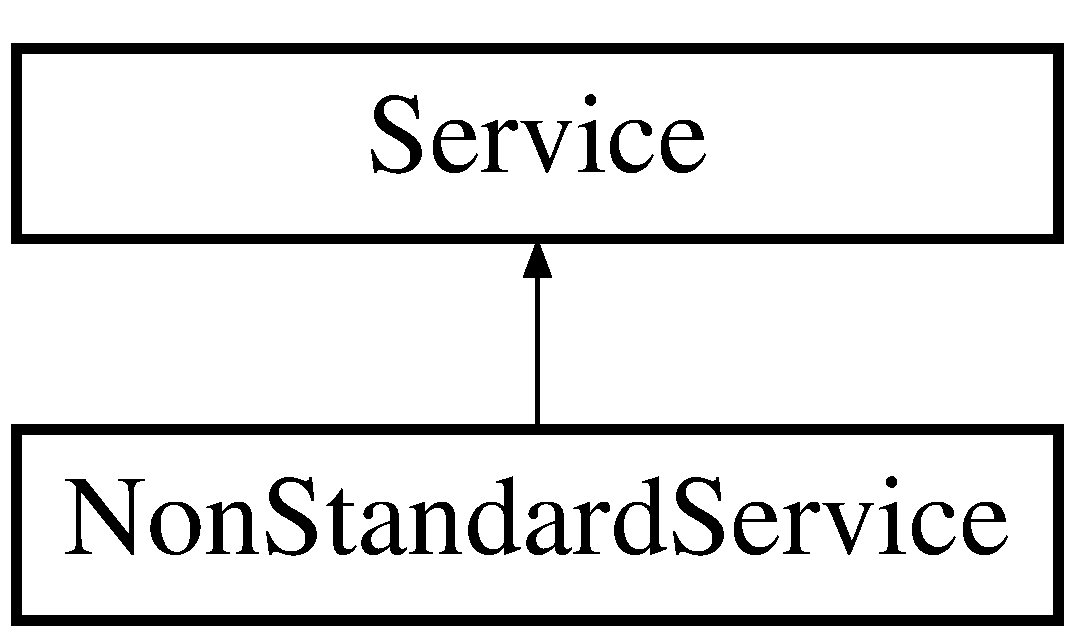
\includegraphics[height=2.000000cm]{class_non_standard_service}
\end{center}
\end{figure}
\subsection*{Public Member Functions}
\begin{DoxyCompactItemize}
\item 
\hypertarget{class_non_standard_service_a3eeab361bd1dc205e4a6abb144af66bf}{}{\bfseries Non\+Standard\+Service} (\hyperlink{struct_date}{Date} starting\+Date, string description, float price, int duration)\label{class_non_standard_service_a3eeab361bd1dc205e4a6abb144af66bf}

\item 
\hypertarget{class_non_standard_service_a669ba4a8b566d49e664f8b4490a41ef6}{}{\bfseries Non\+Standard\+Service} (istream \&in)\label{class_non_standard_service_a669ba4a8b566d49e664f8b4490a41ef6}

\item 
\hypertarget{class_non_standard_service_aa2dc386947829a1bb0ebf10b659346d2}{}int {\bfseries class\+Identifier} ()\label{class_non_standard_service_aa2dc386947829a1bb0ebf10b659346d2}

\item 
\hypertarget{class_non_standard_service_a4ceaaf1e9f8793720598fcb94dad64f4}{}void {\bfseries save\+Object\+Info} (ostream \&out)\label{class_non_standard_service_a4ceaaf1e9f8793720598fcb94dad64f4}

\item 
\hypertarget{class_non_standard_service_a610f7f208834c25a431b7b4830a8425f}{}float {\bfseries get\+Price} () const \label{class_non_standard_service_a610f7f208834c25a431b7b4830a8425f}

\item 
\hypertarget{class_non_standard_service_ad445ce9acca0d4f67a46adad0bc91227}{}int {\bfseries get\+Duration} () const \label{class_non_standard_service_ad445ce9acca0d4f67a46adad0bc91227}

\item 
\hypertarget{class_non_standard_service_a5726d3d995c946a13028a3e396dac2ab}{}const string \& {\bfseries get\+Description} () const \label{class_non_standard_service_a5726d3d995c946a13028a3e396dac2ab}

\end{DoxyCompactItemize}
\subsection*{Additional Inherited Members}


\subsection{Detailed Description}
Non Standard Services Performed on Vehicles. 

The documentation for this class was generated from the following files\+:\begin{DoxyCompactItemize}
\item 
Service.\+h\item 
Service.\+cpp\end{DoxyCompactItemize}

\hypertarget{class_oil_change}{}\section{Oil\+Change Class Reference}
\label{class_oil_change}\index{Oil\+Change@{Oil\+Change}}


Oil Change \hyperlink{class_service}{Service} Performed on Vehicles.  




{\ttfamily \#include $<$Service.\+h$>$}

Inheritance diagram for Oil\+Change\+:\begin{figure}[H]
\begin{center}
\leavevmode
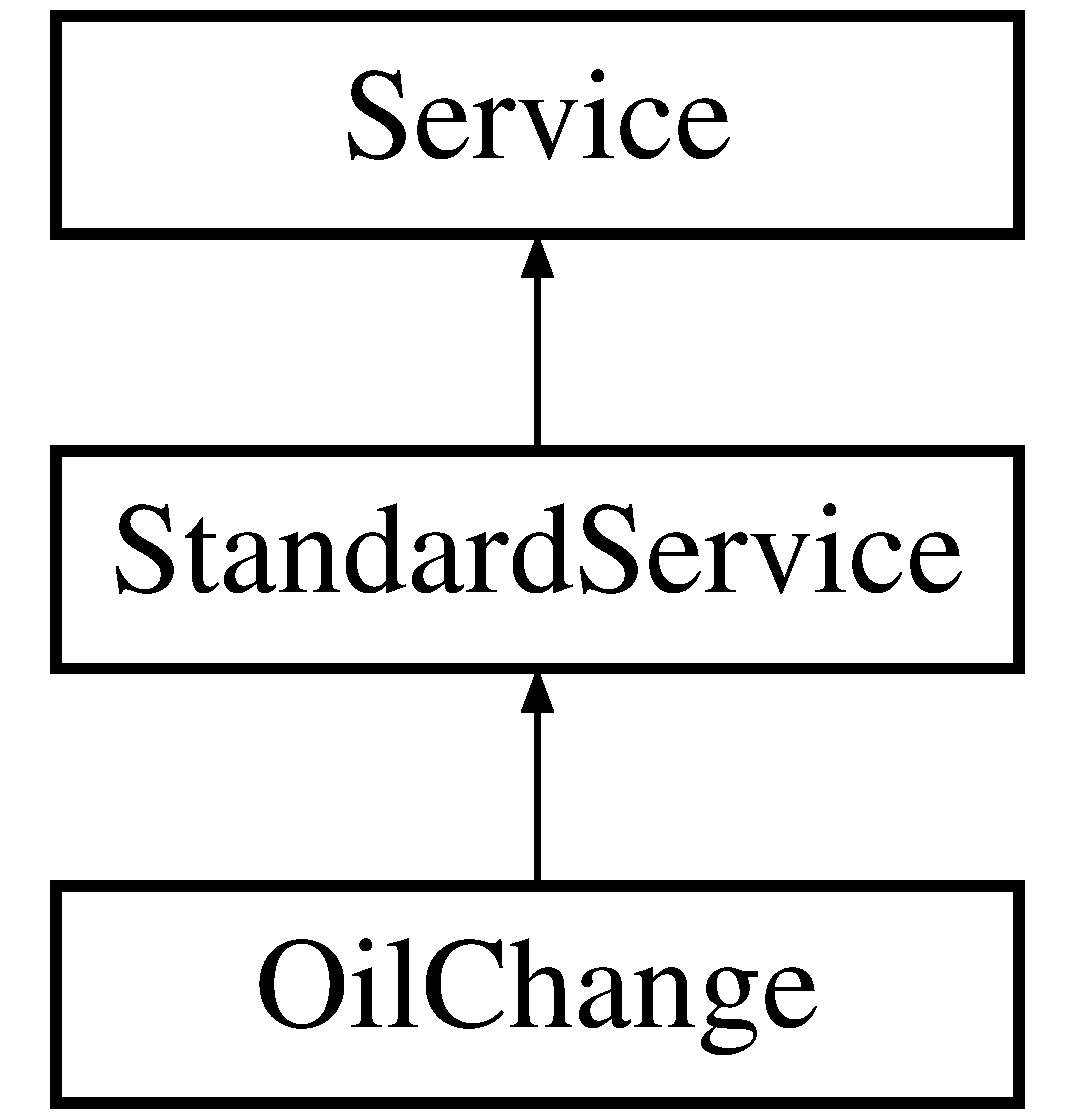
\includegraphics[height=3.000000cm]{class_oil_change}
\end{center}
\end{figure}
\subsection*{Public Member Functions}
\begin{DoxyCompactItemize}
\item 
\hypertarget{class_oil_change_a1383f2d2827ef534c8c37c967283941e}{}{\bfseries Oil\+Change} (\hyperlink{struct_date}{Date} starting\+Date)\label{class_oil_change_a1383f2d2827ef534c8c37c967283941e}

\item 
\hypertarget{class_oil_change_a12a02bc018b33902272a06b31b62c683}{}{\bfseries Oil\+Change} (istream \&in)\label{class_oil_change_a12a02bc018b33902272a06b31b62c683}

\item 
\hypertarget{class_oil_change_a1f6b07d29276ce9fd0378b99345a4757}{}int {\bfseries class\+Identifier} ()\label{class_oil_change_a1f6b07d29276ce9fd0378b99345a4757}

\item 
\hypertarget{class_oil_change_a860cd72ae2a2bcad46d13ca7aadc8218}{}void {\bfseries save\+Object\+Info} (ostream \&out)\label{class_oil_change_a860cd72ae2a2bcad46d13ca7aadc8218}

\item 
\hypertarget{class_oil_change_a57566c0c32f7891ab35639fe8d0167db}{}float {\bfseries get\+Price} () const \label{class_oil_change_a57566c0c32f7891ab35639fe8d0167db}

\item 
\hypertarget{class_oil_change_a77b7cde26a4b6e21d4edec722cd1301c}{}int {\bfseries get\+Duration} () const \label{class_oil_change_a77b7cde26a4b6e21d4edec722cd1301c}

\item 
\hypertarget{class_oil_change_a9f5619aa6259abe36edee2ff4809ae10}{}const string \& {\bfseries get\+Description} () const \label{class_oil_change_a9f5619aa6259abe36edee2ff4809ae10}

\end{DoxyCompactItemize}
\subsection*{Additional Inherited Members}


\subsection{Detailed Description}
Oil Change \hyperlink{class_service}{Service} Performed on Vehicles. 

\hyperlink{class_inspection}{Inspection} \hyperlink{class_service}{Service} Performed on Vehicles. 

The documentation for this class was generated from the following files\+:\begin{DoxyCompactItemize}
\item 
Service.\+h\item 
Service.\+cpp\end{DoxyCompactItemize}

\hypertarget{class_person}{}\section{Person Class Reference}
\label{class_person}\index{Person@{Person}}


Superclass to \hyperlink{class_employee}{Employee} and \hyperlink{class_client}{Client}.  




{\ttfamily \#include $<$Auto\+Repair\+Shop.\+h$>$}

Inheritance diagram for Person\+:\begin{figure}[H]
\begin{center}
\leavevmode
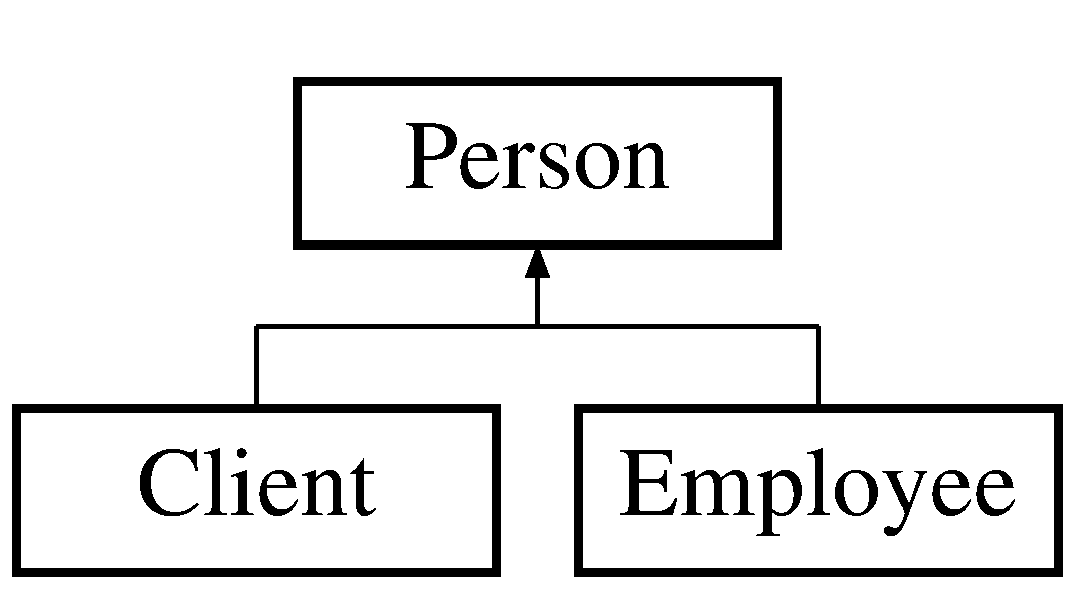
\includegraphics[height=2.000000cm]{class_person}
\end{center}
\end{figure}
\subsection*{Public Member Functions}
\begin{DoxyCompactItemize}
\item 
\hypertarget{class_person_aba0adcb7be258cfdda603c6261a61985}{}\hyperlink{class_person_aba0adcb7be258cfdda603c6261a61985}{Person} (string name)\label{class_person_aba0adcb7be258cfdda603c6261a61985}

\begin{DoxyCompactList}\small\item\em creates an object of \hyperlink{class_person}{Person} class \end{DoxyCompactList}\item 
\hyperlink{class_person_a748e7012f90b5d9666687b15a4b5bd7f}{Person} (istream \&in, string name, vector$<$ string $>$ \&license\+Plates)
\begin{DoxyCompactList}\small\item\em reads an object of \hyperlink{class_person}{Person} class from a stream \end{DoxyCompactList}\item 
\hypertarget{class_person_aba5495c75e9294a1dcd7a0624d8f7fc2}{}void \hyperlink{class_person_aba5495c75e9294a1dcd7a0624d8f7fc2}{save\+Object\+Info} (ostream \&out)\label{class_person_aba5495c75e9294a1dcd7a0624d8f7fc2}

\begin{DoxyCompactList}\small\item\em saves the objects\textquotesingle{} info to a stream \end{DoxyCompactList}\item 
\hypertarget{class_person_a7f14c8d2bc2b51b3304085689b021b33}{}virtual void \hyperlink{class_person_a7f14c8d2bc2b51b3304085689b021b33}{print\+Object\+Info} () const \label{class_person_a7f14c8d2bc2b51b3304085689b021b33}

\begin{DoxyCompactList}\small\item\em prints the objects\textquotesingle{} info to std\+::cout \end{DoxyCompactList}\item 
\hypertarget{class_person_a3776df9441e6a8f7165948d893e2c027}{}bool \hyperlink{class_person_a3776df9441e6a8f7165948d893e2c027}{add\+Vehicle} (\hyperlink{class_vehicle}{Vehicle} $\ast$vehicle)\label{class_person_a3776df9441e6a8f7165948d893e2c027}

\begin{DoxyCompactList}\small\item\em adds a vehicle to the person\textquotesingle{}s vector of vehicles \end{DoxyCompactList}\item 
\hypertarget{class_person_ae804590441c0a4057c3e4a9912393f12}{}bool \hyperlink{class_person_ae804590441c0a4057c3e4a9912393f12}{remove\+Vehicle} (\hyperlink{class_vehicle}{Vehicle} $\ast$vehicle)\label{class_person_ae804590441c0a4057c3e4a9912393f12}

\begin{DoxyCompactList}\small\item\em removes a vehicle from the person\textquotesingle{}s vector of vehicles \end{DoxyCompactList}\item 
\hypertarget{class_person_aef412cfd816a9ffc60f6c99a9dc58dc1}{}void \hyperlink{class_person_aef412cfd816a9ffc60f6c99a9dc58dc1}{set\+I\+D} (int id)\label{class_person_aef412cfd816a9ffc60f6c99a9dc58dc1}

\begin{DoxyCompactList}\small\item\em sets the person I\+D to the given value \end{DoxyCompactList}\item 
int \hyperlink{class_person_a7ed80c648874ad61eb3f482ea50b1f26}{get\+I\+D} () const 
\item 
string \hyperlink{class_person_a5c06a41731a2656caec65e3bc39f5ebe}{get\+Name} () const 
\item 
vector$<$ \hyperlink{class_vehicle}{Vehicle} $\ast$ $>$ \hyperlink{class_person_abbf0a20a74ada90543dff88e9b0d6064}{get\+Vehicles} () const 
\end{DoxyCompactItemize}
\subsection*{Protected Attributes}
\begin{DoxyCompactItemize}
\item 
\hypertarget{class_person_a669b64897b4d823a27bb5866368d4dfa}{}string {\bfseries name}\label{class_person_a669b64897b4d823a27bb5866368d4dfa}

\item 
\hypertarget{class_person_a79076878abcbbdf33ff49e2dcb55b043}{}vector$<$ \hyperlink{class_vehicle}{Vehicle} $\ast$ $>$ {\bfseries vehicles}\label{class_person_a79076878abcbbdf33ff49e2dcb55b043}

\item 
\hypertarget{class_person_aec48a92f614a854ff380a15eb8e2f479}{}int {\bfseries id}\label{class_person_aec48a92f614a854ff380a15eb8e2f479}

\end{DoxyCompactItemize}


\subsection{Detailed Description}
Superclass to \hyperlink{class_employee}{Employee} and \hyperlink{class_client}{Client}. 

\subsection{Constructor \& Destructor Documentation}
\hypertarget{class_person_a748e7012f90b5d9666687b15a4b5bd7f}{}\index{Person@{Person}!Person@{Person}}
\index{Person@{Person}!Person@{Person}}
\subsubsection[{Person(istream \&in, string name, vector$<$ string $>$ \&license\+Plates)}]{\setlength{\rightskip}{0pt plus 5cm}Person\+::\+Person (
\begin{DoxyParamCaption}
\item[{istream \&}]{in, }
\item[{string}]{name, }
\item[{vector$<$ string $>$ \&}]{license\+Plates}
\end{DoxyParamCaption}
)}\label{class_person_a748e7012f90b5d9666687b15a4b5bd7f}


reads an object of \hyperlink{class_person}{Person} class from a stream 


\begin{DoxyParams}[1]{Parameters}
\mbox{\tt out}  & {\em license\+Plates} & returns the license plates of all vehicles related to \hyperlink{class_person}{Person} \\
\hline
\end{DoxyParams}


\subsection{Member Function Documentation}
\hypertarget{class_person_a7ed80c648874ad61eb3f482ea50b1f26}{}\index{Person@{Person}!get\+I\+D@{get\+I\+D}}
\index{get\+I\+D@{get\+I\+D}!Person@{Person}}
\subsubsection[{get\+I\+D() const }]{\setlength{\rightskip}{0pt plus 5cm}int Person\+::get\+I\+D (
\begin{DoxyParamCaption}
{}
\end{DoxyParamCaption}
) const\hspace{0.3cm}{\ttfamily [inline]}}\label{class_person_a7ed80c648874ad61eb3f482ea50b1f26}
\begin{DoxyReturn}{Returns}
the person\textquotesingle{}s I\+D 
\end{DoxyReturn}
\hypertarget{class_person_a5c06a41731a2656caec65e3bc39f5ebe}{}\index{Person@{Person}!get\+Name@{get\+Name}}
\index{get\+Name@{get\+Name}!Person@{Person}}
\subsubsection[{get\+Name() const }]{\setlength{\rightskip}{0pt plus 5cm}string Person\+::get\+Name (
\begin{DoxyParamCaption}
{}
\end{DoxyParamCaption}
) const\hspace{0.3cm}{\ttfamily [inline]}}\label{class_person_a5c06a41731a2656caec65e3bc39f5ebe}
\begin{DoxyReturn}{Returns}
the person\textquotesingle{}s name 
\end{DoxyReturn}
\hypertarget{class_person_abbf0a20a74ada90543dff88e9b0d6064}{}\index{Person@{Person}!get\+Vehicles@{get\+Vehicles}}
\index{get\+Vehicles@{get\+Vehicles}!Person@{Person}}
\subsubsection[{get\+Vehicles() const }]{\setlength{\rightskip}{0pt plus 5cm}vector$<${\bf Vehicle} $\ast$$>$ Person\+::get\+Vehicles (
\begin{DoxyParamCaption}
{}
\end{DoxyParamCaption}
) const\hspace{0.3cm}{\ttfamily [inline]}}\label{class_person_abbf0a20a74ada90543dff88e9b0d6064}
\begin{DoxyReturn}{Returns}
the person\textquotesingle{}s vehicle vector 
\end{DoxyReturn}


The documentation for this class was generated from the following files\+:\begin{DoxyCompactItemize}
\item 
Auto\+Repair\+Shop.\+h\item 
Auto\+Repair\+Shop.\+cpp\end{DoxyCompactItemize}

\hypertarget{class_service}{}\section{Service Class Reference}
\label{class_service}\index{Service@{Service}}


superclass to \hyperlink{class_standard_service}{Standard\+Service} and \hyperlink{class_non_standard_service}{Non\+Standard\+Service}  




{\ttfamily \#include $<$Service.\+h$>$}

Inheritance diagram for Service\+:\begin{figure}[H]
\begin{center}
\leavevmode
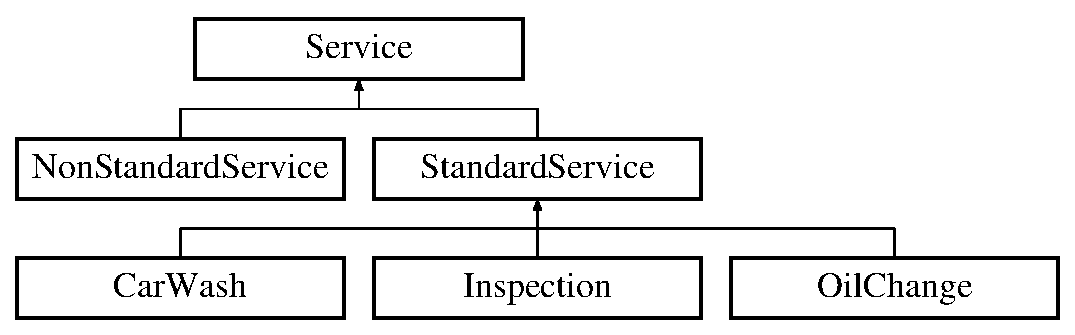
\includegraphics[height=3.000000cm]{class_service}
\end{center}
\end{figure}
\subsection*{Public Member Functions}
\begin{DoxyCompactItemize}
\item 
\hypertarget{class_service_a70b17e468ca513b3d379b81349614594}{}{\bfseries Service} (\hyperlink{struct_date}{Date} starting\+Date)\label{class_service_a70b17e468ca513b3d379b81349614594}

\item 
\hypertarget{class_service_ada80b8d4356fb275d1b45777b08f2d00}{}{\bfseries Service} (istream \&in)\label{class_service_ada80b8d4356fb275d1b45777b08f2d00}

\item 
\hypertarget{class_service_a55a7bfff43a2cf1fad22749475be2bc4}{}virtual int {\bfseries class\+Identifier} ()\label{class_service_a55a7bfff43a2cf1fad22749475be2bc4}

\item 
\hypertarget{class_service_a3f7311721c3bced9b3effec67ac50319}{}virtual void {\bfseries save\+Object\+Info} (ostream \&out)\label{class_service_a3f7311721c3bced9b3effec67ac50319}

\item 
\hypertarget{class_service_ac89fe4d9ab6fcf8e42e85e5f4d6f9fb9}{}void {\bfseries print\+Object\+Info} ()\label{class_service_ac89fe4d9ab6fcf8e42e85e5f4d6f9fb9}

\item 
\hypertarget{class_service_a054bc119ce47bf2ca559f14bbdfe1ee4}{}virtual float {\bfseries get\+Price} () const  =0\label{class_service_a054bc119ce47bf2ca559f14bbdfe1ee4}

\item 
\hypertarget{class_service_a31d668e91f3b357f892bfb8a50840fdb}{}virtual int {\bfseries get\+Duration} () const  =0\label{class_service_a31d668e91f3b357f892bfb8a50840fdb}

\item 
\hypertarget{class_service_a666263257ab2bdbd270fbeb34f1edbd3}{}virtual const string \& {\bfseries get\+Description} () const  =0\label{class_service_a666263257ab2bdbd270fbeb34f1edbd3}

\item 
\hypertarget{class_service_a6977a78bac9e8007b24baec0ff3ce01e}{}\hyperlink{struct_date}{Date} {\bfseries get\+Starting\+Date} () const \label{class_service_a6977a78bac9e8007b24baec0ff3ce01e}

\end{DoxyCompactItemize}
\subsection*{Protected Attributes}
\begin{DoxyCompactItemize}
\item 
\hypertarget{class_service_a412240629a97315e5005770c0c965d6d}{}string {\bfseries description}\label{class_service_a412240629a97315e5005770c0c965d6d}

\item 
\hypertarget{class_service_a7daf7b57889f8147767ed185468ed202}{}float {\bfseries price}\label{class_service_a7daf7b57889f8147767ed185468ed202}

\item 
\hypertarget{class_service_a7b13f5323bb580051ced9b976c41d3b0}{}\hyperlink{struct_date}{Date} {\bfseries starting\+Date}\label{class_service_a7b13f5323bb580051ced9b976c41d3b0}

\item 
\hypertarget{class_service_a001abaecc2ecdcd962f5687a025f81da}{}int {\bfseries duration}\label{class_service_a001abaecc2ecdcd962f5687a025f81da}

\end{DoxyCompactItemize}


\subsection{Detailed Description}
superclass to \hyperlink{class_standard_service}{Standard\+Service} and \hyperlink{class_non_standard_service}{Non\+Standard\+Service} 

The documentation for this class was generated from the following files\+:\begin{DoxyCompactItemize}
\item 
Service.\+h\item 
Service.\+cpp\end{DoxyCompactItemize}

\hypertarget{class_standard_service}{}\section{Standard\+Service Class Reference}
\label{class_standard_service}\index{Standard\+Service@{Standard\+Service}}


superclass to \hyperlink{class_oil_change}{Oil\+Change}, \hyperlink{class_inspection}{Inspection} and \hyperlink{class_car_wash}{Car\+Wash}  




{\ttfamily \#include $<$Service.\+h$>$}

Inheritance diagram for Standard\+Service\+:\begin{figure}[H]
\begin{center}
\leavevmode
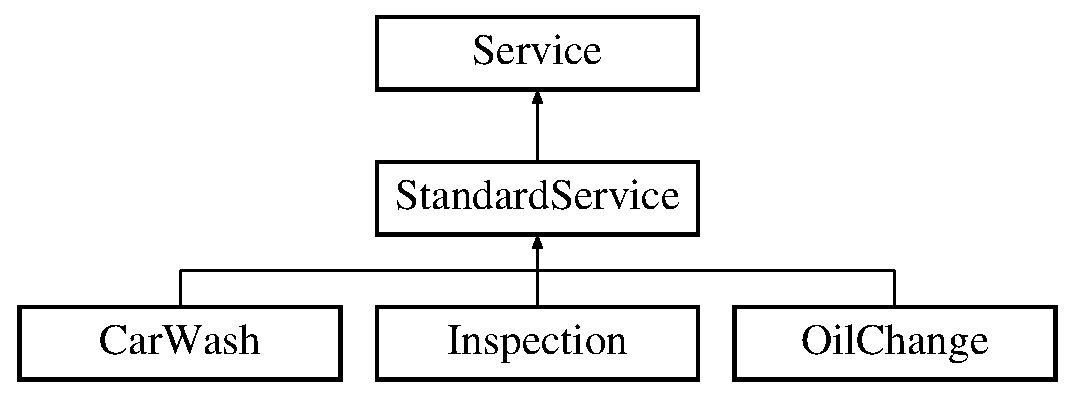
\includegraphics[height=3.000000cm]{class_standard_service}
\end{center}
\end{figure}
\subsection*{Public Member Functions}
\begin{DoxyCompactItemize}
\item 
\hypertarget{class_standard_service_aa5adb06b6c2253879530879fe38b8f92}{}{\bfseries Standard\+Service} (\hyperlink{struct_date}{Date} starting\+Date)\label{class_standard_service_aa5adb06b6c2253879530879fe38b8f92}

\item 
\hypertarget{class_standard_service_a0ab11433e170d74a684c50c21b6d35cf}{}{\bfseries Standard\+Service} (istream \&in)\label{class_standard_service_a0ab11433e170d74a684c50c21b6d35cf}

\item 
\hypertarget{class_standard_service_ae5b28b6a444f0bf5a60a7acd030a1368}{}virtual int {\bfseries class\+Identifier} ()\label{class_standard_service_ae5b28b6a444f0bf5a60a7acd030a1368}

\item 
\hypertarget{class_standard_service_a7fcb88363b52004585e7f3548b864927}{}virtual void {\bfseries save\+Object\+Info} (ostream \&out)\label{class_standard_service_a7fcb88363b52004585e7f3548b864927}

\end{DoxyCompactItemize}
\subsection*{Additional Inherited Members}


\subsection{Detailed Description}
superclass to \hyperlink{class_oil_change}{Oil\+Change}, \hyperlink{class_inspection}{Inspection} and \hyperlink{class_car_wash}{Car\+Wash} 

The documentation for this class was generated from the following file\+:\begin{DoxyCompactItemize}
\item 
Service.\+h\end{DoxyCompactItemize}

\hypertarget{class_truck}{}\section{Truck Class Reference}
\label{class_truck}\index{Truck@{Truck}}
Inheritance diagram for Truck\+:\begin{figure}[H]
\begin{center}
\leavevmode
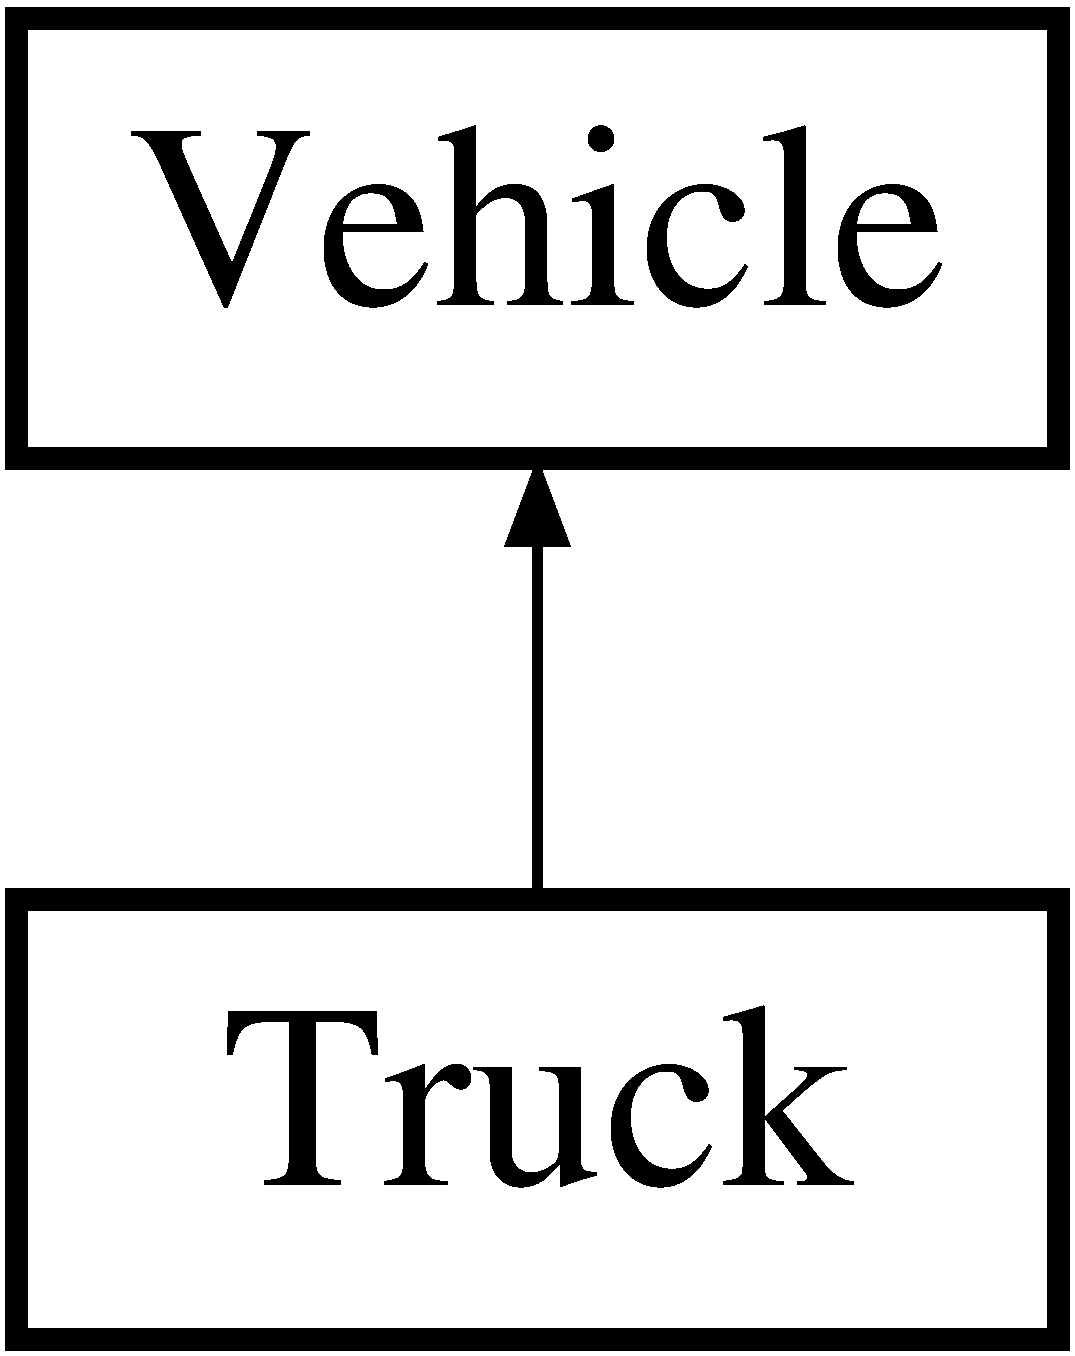
\includegraphics[height=2.000000cm]{class_truck}
\end{center}
\end{figure}
\subsection*{Public Member Functions}
\begin{DoxyCompactItemize}
\item 
\hypertarget{class_truck_a0a8dd0074ba97cb9c9e4a85c1940f487}{}{\bfseries Truck} (string manufacturer, string model, string license\+Plate, int max\+Weight)\label{class_truck_a0a8dd0074ba97cb9c9e4a85c1940f487}

\item 
\hypertarget{class_truck_a5cfc074de127de059181b8b36c45ff63}{}{\bfseries Truck} (istream \&in)\label{class_truck_a5cfc074de127de059181b8b36c45ff63}

\item 
\hypertarget{class_truck_a520b836bc6d09157c03edbc8e28b0ae3}{}int {\bfseries class\+Identifier} ()\label{class_truck_a520b836bc6d09157c03edbc8e28b0ae3}

\item 
\hypertarget{class_truck_a05acb002a6530883dcfaf5b652108c7e}{}void {\bfseries save\+Object\+Info} (ostream \&out)\label{class_truck_a05acb002a6530883dcfaf5b652108c7e}

\item 
\hypertarget{class_truck_add59302c411d863d9fc8be4a91fe74b2}{}void {\bfseries print\+Object\+Info} () const \label{class_truck_add59302c411d863d9fc8be4a91fe74b2}

\end{DoxyCompactItemize}


The documentation for this class was generated from the following files\+:\begin{DoxyCompactItemize}
\item 
Vehicle.\+h\item 
Vehicle.\+cpp\end{DoxyCompactItemize}

\hypertarget{class_vehicle}{}\section{Vehicle Class Reference}
\label{class_vehicle}\index{Vehicle@{Vehicle}}


superclass to \hyperlink{class_automobile}{Automobile}, \hyperlink{class_motorcycle}{Motorcycle}, \hyperlink{class_truck}{Truck} and \hyperlink{class_bus}{Bus}  




{\ttfamily \#include $<$Vehicle.\+h$>$}

Inheritance diagram for Vehicle\+:\begin{figure}[H]
\begin{center}
\leavevmode
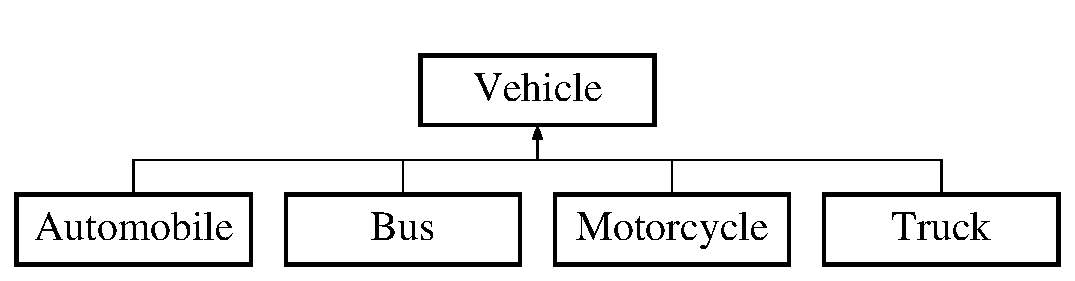
\includegraphics[height=2.000000cm]{class_vehicle}
\end{center}
\end{figure}
\subsection*{Public Member Functions}
\begin{DoxyCompactItemize}
\item 
\hypertarget{class_vehicle_a893b8305e67b405820374681ca24adb8}{}{\bfseries Vehicle} (string manufacturer, string model, string license\+Plate)\label{class_vehicle_a893b8305e67b405820374681ca24adb8}

\item 
\hypertarget{class_vehicle_a9c1e962253f1caf699b72e9081d8c02c}{}{\bfseries Vehicle} (istream \&in)\label{class_vehicle_a9c1e962253f1caf699b72e9081d8c02c}

\item 
\hypertarget{class_vehicle_a156149accbe781d1533ac3326f8b8c36}{}virtual int {\bfseries class\+Identifier} ()\label{class_vehicle_a156149accbe781d1533ac3326f8b8c36}

\item 
\hypertarget{class_vehicle_abe2134da6c7c2dac66634f8bab33d4e0}{}virtual void {\bfseries save\+Object\+Info} (ostream \&out)\label{class_vehicle_abe2134da6c7c2dac66634f8bab33d4e0}

\item 
\hypertarget{class_vehicle_aa0dcd60b0862190b33e03e356e5ac605}{}virtual void {\bfseries print\+Object\+Info} () const \label{class_vehicle_aa0dcd60b0862190b33e03e356e5ac605}

\item 
\hypertarget{class_vehicle_aa8b234215cdebfbcfc0638070cc0055d}{}void {\bfseries print\+Services} () const \label{class_vehicle_aa8b234215cdebfbcfc0638070cc0055d}

\item 
\hypertarget{class_vehicle_a80cf791ce88075cab396cf074636f7c2}{}bool {\bfseries add\+Service} (\hyperlink{class_service}{Service} $\ast$s1)\label{class_vehicle_a80cf791ce88075cab396cf074636f7c2}

\item 
\hypertarget{class_vehicle_aedab174d431748f24e703e151c4208f8}{}bool {\bfseries remove\+Service} (\hyperlink{class_service}{Service} $\ast$s1)\label{class_vehicle_aedab174d431748f24e703e151c4208f8}

\item 
\hypertarget{class_vehicle_a425dc48d7b612ebefe2d62d6ff0a13f8}{}const string \& {\bfseries get\+License\+Plate} () const \label{class_vehicle_a425dc48d7b612ebefe2d62d6ff0a13f8}

\item 
\hypertarget{class_vehicle_a09ebc4c11e1004681ec4d78c93e9013c}{}const string \& {\bfseries get\+Manufacturer} () const \label{class_vehicle_a09ebc4c11e1004681ec4d78c93e9013c}

\item 
\hypertarget{class_vehicle_a5169e58c8510a256438a1b7532aa422f}{}const string \& {\bfseries get\+Model} () const \label{class_vehicle_a5169e58c8510a256438a1b7532aa422f}

\end{DoxyCompactItemize}


\subsection{Detailed Description}
superclass to \hyperlink{class_automobile}{Automobile}, \hyperlink{class_motorcycle}{Motorcycle}, \hyperlink{class_truck}{Truck} and \hyperlink{class_bus}{Bus} 

The documentation for this class was generated from the following files\+:\begin{DoxyCompactItemize}
\item 
Vehicle.\+h\item 
Vehicle.\+cpp\end{DoxyCompactItemize}

\hypertarget{class_vehicles_file}{}\section{Vehicles\+File Class Reference}
\label{class_vehicles_file}\index{Vehicles\+File@{Vehicles\+File}}


contains the info of all the vehicles on the Auto Repair Shop  




{\ttfamily \#include $<$Config\+File.\+h$>$}

Inheritance diagram for Vehicles\+File\+:\begin{figure}[H]
\begin{center}
\leavevmode
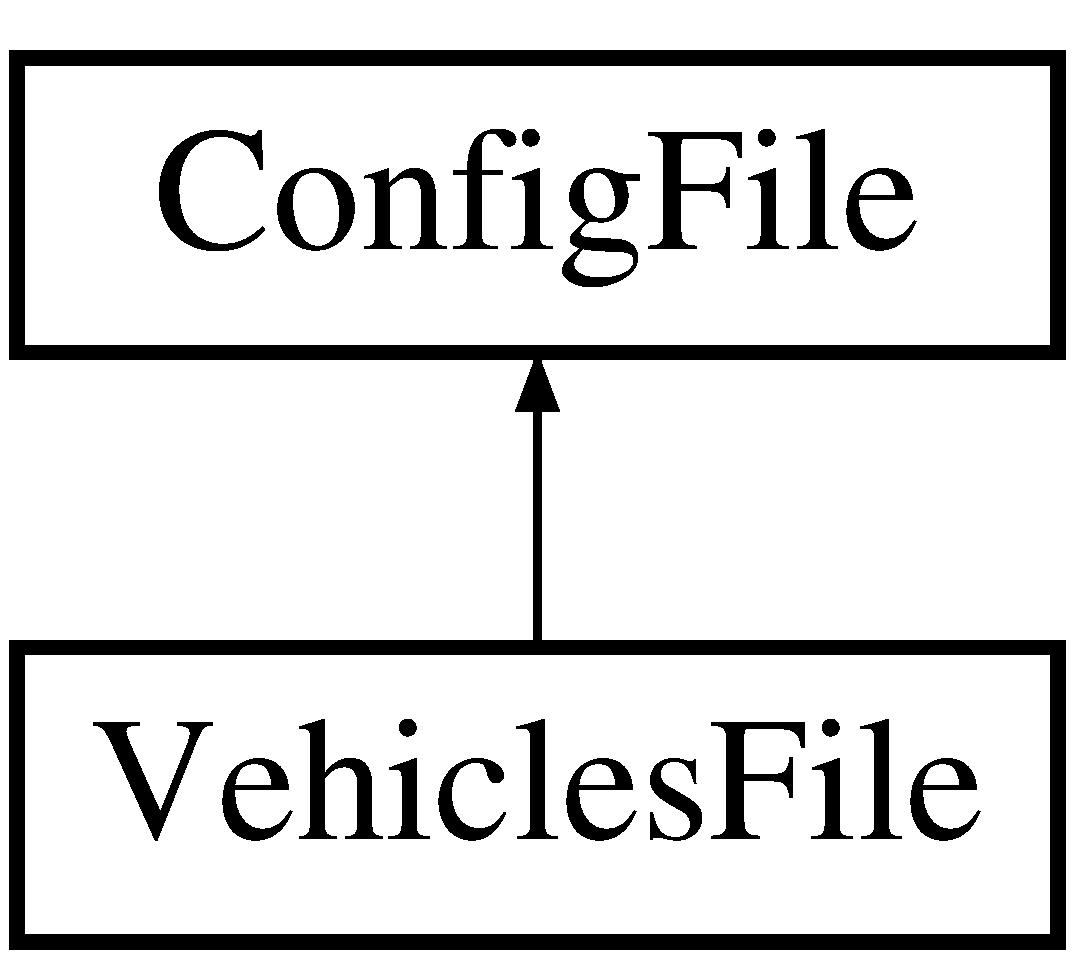
\includegraphics[height=2.000000cm]{class_vehicles_file}
\end{center}
\end{figure}
\subsection*{Public Member Functions}
\begin{DoxyCompactItemize}
\item 
\hypertarget{class_vehicles_file_ab2e1263800fe0705f6c8008e19e611f0}{}{\bfseries Vehicles\+File} (string \&filename)\label{class_vehicles_file_ab2e1263800fe0705f6c8008e19e611f0}

\item 
\hypertarget{class_vehicles_file_afcb5e23825c05522296c543841b85939}{}bool \hyperlink{class_vehicles_file_afcb5e23825c05522296c543841b85939}{save\+Data} (\hyperlink{class_auto_repair_shop}{Auto\+Repair\+Shop} \&repair\+Shop, bool overwrite=false)\label{class_vehicles_file_afcb5e23825c05522296c543841b85939}

\begin{DoxyCompactList}\small\item\em saves the file data \end{DoxyCompactList}\item 
bool \hyperlink{class_vehicles_file_a4299cf7cbc0ce9123d753f0aba2b95cf}{load\+Data} (\hyperlink{class_auto_repair_shop}{Auto\+Repair\+Shop} \&repair\+Shop)
\begin{DoxyCompactList}\small\item\em loads data from the file \end{DoxyCompactList}\end{DoxyCompactItemize}
\subsection*{Additional Inherited Members}


\subsection{Detailed Description}
contains the info of all the vehicles on the Auto Repair Shop 

\subsection{Member Function Documentation}
\hypertarget{class_vehicles_file_a4299cf7cbc0ce9123d753f0aba2b95cf}{}\index{Vehicles\+File@{Vehicles\+File}!load\+Data@{load\+Data}}
\index{load\+Data@{load\+Data}!Vehicles\+File@{Vehicles\+File}}
\subsubsection[{load\+Data(\+Auto\+Repair\+Shop \&repair\+Shop)}]{\setlength{\rightskip}{0pt plus 5cm}bool Vehicles\+File\+::load\+Data (
\begin{DoxyParamCaption}
\item[{{\bf Auto\+Repair\+Shop} \&}]{repair\+Shop}
\end{DoxyParamCaption}
)}\label{class_vehicles_file_a4299cf7cbc0ce9123d753f0aba2b95cf}


loads data from the file 

\begin{DoxyReturn}{Returns}
false if the file doesn\textquotesingle{}t exist 
\end{DoxyReturn}


The documentation for this class was generated from the following files\+:\begin{DoxyCompactItemize}
\item 
Config\+File.\+h\item 
Config\+File.\+cpp\end{DoxyCompactItemize}

%--- End generated contents ---

% Index
\backmatter
\newpage
\phantomsection
\clearemptydoublepage
\addcontentsline{toc}{chapter}{Index}
\printindex

\end{document}
